\documentclass{beamer}
\usecolortheme{dove}
\setbeamertemplate{navigation symbols}{}
\newenvironment{alltt}{\ttfamily}{\par}
\usepackage{amsmath,amssymb,amsfonts,amsthm, multicol, subfigure, color}
\usepackage{bm}
\usepackage{graphicx}
\usepackage{tabularx}
\usepackage{booktabs}
\usepackage{hyperref}
\usepackage{pdfpages}
\usepackage{xcolor}
\definecolor{dodgerblue}{rgb}{.118, .575, 1}
\definecolor{seagreen4}{RGB}{46, 139, 87}
\def\independenT#1#2{\mathrel{\rlap{$#1#2$}\mkern2mu{#1#2}}}
\newcommand\independent{\protect\mathpalette{\protect\independenT}{\perp}}
\newcommand\indep{\protect\mathpalette{\protect\independenT}{\perp}}
\def\logit{\text{logit}}
\usepackage{stackrel}
\usepackage{tikz}
\usetikzlibrary{arrows,shapes.arrows,positioning,shapes,patterns,calc}
\newcommand\slideref[1]{\vskip .1cm \scriptsize \textcolor{gray}{{#1}}}
\definecolor{seagreen}{RGB}{46, 139, 87}
\newcommand\red[1]{\color{red}#1}
\newcommand\blue[1]{\color{blue}#1}
\newcommand\gray[1]{\color{gray}#1}
\newcommand\green[1]{\color{olive}#1}
\newcommand\seagreen[1]{\color{seagreen}#1}
\newcommand\purple[1]{\color{purple}#1}
\newcommand\orange[1]{\color{orange}#1}
\newcommand\black[1]{\color{black}#1}
\newcommand\white[1]{\color{white}#1}
\newcommand\teal[1]{\color{teal}#1}
\newcommand\magenta[1]{\color{magenta}#1}
\newcommand\Fuchsia[1]{\color{Fuchsia}#1}
\newcommand\BlueGreen[1]{\color{BlueGreen}#1}
\newcommand\bblue[1]{\textcolor{blue}{\textbf{#1}}}
\newcommand\bred[1]{\textcolor{red}{\textbf{#1}}}
\newcommand\bgray[1]{\textcolor{gray}{\textbf{#1}}}
\newcommand\bgreen[1]{\textcolor{seagreen}{\textbf{#1}}}
\colorlet{lightgray}{gray!40}
\pgfdeclarelayer{bg}    % declare background layer for tikz
\pgfsetlayers{bg,main} % order layers for tikz
\newcommand\bref[2]{\href{#1}{\color{blue}{#2}}}
\newcommand\mycite[1]{\begin{scriptsize}\textcolor{darkgray}{(#1)}\end{scriptsize}}
\newcommand\iid{\stackrel{\text{iid}}{\sim}}
\newcommand\E{\text{E}}
\newcommand\V{\text{V}}
\renewcommand\P{\text{P}}
\newcommand{\Cov}{\text{Cov}}
\newcommand{\Cor}{\text{Cor}}
\newcommand\doop{\text{do}}
\newcommand{\tcframe}{\frame{
\small{
\only<1|handout:0>{\tableofcontents}
\only<2|handout:1>{\tableofcontents[currentsection]}}
}}
% Credit for the following to https://tex.stackexchange.com/questions/44983/beamer-removing-headline-and-its-space-on-a-single-frame-for-plan-but-keepin
\makeatletter
    \newenvironment{withoutheadline}{
        \setbeamertemplate{headline}[default]
        \def\beamer@entrycode{\vspace*{-\headheight}}
    }{}
\makeatother
\setbeamercovered{invisible}
\usepackage[round]{natbib}
\bibliographystyle{humannat-mod}
\setbeamertemplate{enumerate items}[default]
\usepackage{mathtools}
% BELOW THREE LINES MAKES NAME IN FOOTER
\setbeamertemplate{footline}[text line]{%
\parbox{\linewidth}{\vspace*{-8pt}Lundberg, Johnson, and Stewart. What is Your Estimand?}}%\hfill\insertshortauthor\hfill\insertpagenumber}}

%\setbeamertemplate{footline}[text line]{%
%\parbox{\linewidth}{\vspace*{-8pt}Ian Lundberg (Princeton)}}%\hfill\insertshortauthor\hfill\insertpagenumber}}
%t\setbeamertemplate{navigation symbols}{}

% Make the header figure that will appear frequently
\newcommand\headerfigure{
\begin{tikzpicture}[x = \textwidth, y = \textheight, every node/.style={anchor = center}]
\node at (0,1) {\resizebox{\textwidth}{!}{\begin{tikzpicture}[x = 1.7in, y = .3in]
    \node[cloud, draw, align=center, cloud puffs=20,cloud puff arc=110, aspect=2, inner sep=.5mm, font = \small] (general) at (-.1,0) {Theory or\\general goal};
    %%%%%%%%%%
    \node[align=center, font = \small] (theoretical) at (1,0) {Theoretical\\estimand};
    \draw[->, thick] (general) -- (theoretical);
    \node[align = center, anchor = south, font = {\bf\small}] at (.5,0) {Set};
    \node[align = center, anchor = north, font = \small] at (.5,0) {by argument};
    %%%%%%%%%%
    \node[align=center, font = \small] (empirical) at (2,0) {Empirical\\estimand};
    \draw[->, thick] (theoretical) -- (empirical);
    \node[align = center, anchor = south, font = {\bf\small}] at (1.5,0) {Link};
    \node[align = center, anchor = north, font = \small] at (1.5,0) {by assumption};
    %%%%%%%%%%
    \node[align=center, font = \small] (estimate) at (3,0) {Estimation\\strategy};
    \draw[->, thick] (empirical) -- (estimate);
    \node[align = center, anchor = south, font = {\bf\small}] at (2.5,0) {Learn};
    \node[align = center, anchor = north, font = \small] at (2.5,0) {by data};
    \end{tikzpicture}
    }};
\end{tikzpicture}
}
% Make the versions that have only one step in black
\newcommand\headerfigureset{
\begin{tikzpicture}[x = \textwidth, y = \textheight, every node/.style={anchor = center}]
\node at (0,1) {\resizebox{\textwidth}{!}{\begin{tikzpicture}[x = 1.7in, y = .3in]
    \node[cloud, draw, align=center, cloud puffs=20,cloud puff arc=110, aspect=2, inner sep=.5mm, font = \small] (general) at (-.1,0) {Theory or\\general goal};
    %%%%%%%%%%
    \node[align=center, font = \small] (theoretical) at (1,0) {Theoretical\\estimand};
    \draw[->, thick] (general) -- (theoretical);
    \node[align = center, anchor = south, font = {\bf\small}] at (.5,0) {Set};
    \node[align = center, anchor = north, font = \small] at (.5,0) {by argument};
    %%%%%%%%%%
    \node[align=center, font = \small, gray] (empirical) at (2,0) {Empirical\\estimand};
    \draw[->, thick, gray] (theoretical) -- (empirical);
    \node[align = center, anchor = south, font = {\bf\small}, gray] at (1.5,0) {Link};
    \node[align = center, anchor = north, font = \small, gray] at (1.5,0) {by assumption};
    %%%%%%%%%%
    \node[align=center, font = \small, gray] (estimate) at (3,0) {Estimation\\strategy};
    \draw[->, thick, gray] (empirical) -- (estimate);
    \node[align = center, anchor = south, font = {\bf\small}, gray] at (2.5,0) {Learn};
    \node[align = center, anchor = north, font = \small, gray] at (2.5,0) {by data};
    \end{tikzpicture}
    }};
\end{tikzpicture}
}
\newcommand\headerfigurelink{
\begin{tikzpicture}[x = \textwidth, y = \textheight, every node/.style={anchor = center}]
\node at (0,1) {\resizebox{\textwidth}{!}{\begin{tikzpicture}[x = 1.7in, y = .3in]
    \node[cloud, draw, align=center, cloud puffs=20,cloud puff arc=110, aspect=2, inner sep=.5mm, font = \small, gray] (general) at (-.1,0) {Theory or\\general goal};
    %%%%%%%%%%
    \node[align=center, font = \small] (theoretical) at (1,0) {Theoretical\\estimand};
    \draw[->, thick, gray] (general) -- (theoretical);
    \node[align = center, anchor = south, font = {\bf\small}, gray] at (.5,0) {Set};
    \node[align = center, anchor = north, font = \small, gray] at (.5,0) {by argument};
    %%%%%%%%%%
    \node[align=center, font = \small] (empirical) at (2,0) {Empirical\\estimand};
    \draw[->, thick] (theoretical) -- (empirical);
    \node[align = center, anchor = south, font = {\bf\small}] at (1.5,0) {Link};
    \node[align = center, anchor = north, font = \small] at (1.5,0) {by assumption};
    %%%%%%%%%%
    \node[align=center, font = \small, gray] (estimate) at (3,0) {Estimation\\strategy};
    \draw[->, thick, gray] (empirical) -- (estimate);
    \node[align = center, anchor = south, font = {\bf\small}, gray] at (2.5,0) {Learn};
    \node[align = center, anchor = north, font = \small, gray] at (2.5,0) {by data};
    \end{tikzpicture}
    }};
\end{tikzpicture}
}
\newcommand\headerfigurelearn{
\begin{tikzpicture}[x = \textwidth, y = \textheight, every node/.style={anchor = center}]
\node at (0,1) {\resizebox{\textwidth}{!}{\begin{tikzpicture}[x = 1.7in, y = .3in]
    \node[cloud, draw, align=center, cloud puffs=20,cloud puff arc=110, aspect=2, inner sep=.5mm, font = \small, gray] (general) at (-.1,0) {Theory or\\general goal};
    %%%%%%%%%%
    \node[align=center, font = \small, gray] (theoretical) at (1,0) {Theoretical\\estimand};
    \draw[->, thick, gray] (general) -- (theoretical);
    \node[align = center, anchor = south, font = {\bf\small}, gray] at (.5,0) {Set};
    \node[align = center, anchor = north, font = \small, gray] at (.5,0) {by argument};
    %%%%%%%%%%
    \node[align=center, font = \small] (empirical) at (2,0) {Empirical\\estimand};
    \draw[->, thick, gray] (theoretical) -- (empirical);
    \node[align = center, anchor = south, font = {\bf\small}, gray] at (1.5,0) {Link};
    \node[align = center, anchor = north, font = \small, gray] at (1.5,0) {by assumption};
    %%%%%%%%%%
    \node[align=center, font = \small] (estimate) at (3,0) {Estimation\\strategy};
    \draw[->, thick] (empirical) -- (estimate);
    \node[align = center, anchor = south, font = {\bf\small}] at (2.5,0) {Learn};
    \node[align = center, anchor = north, font = \small] at (2.5,0) {by data};
    \end{tikzpicture}
    }};
\end{tikzpicture}
}

\newcommand\estimandFigure{

\begin{tikzpicture}[x = \textwidth, y = \textheight, every node/.style={anchor = center}]
%\node at (0,1) {\resizebox{\textwidth}{!}{\begin{tikzpicture}[x = 1.7in, y = .3in]
\node<10->[circle, fill = lightgray, draw = lightgray, font = \footnotesize, inner sep = 8pt] (point1) at (.18,.55) {};
\node<10->[gray, font = \footnotesize, align = center, anchor = north] (usqNote) at (point1.south) {A \bgray{unit-specific}\\\bgray{quantity}};
\node[circle, fill = lightgray, draw = lightgray, font = \footnotesize, inner sep = 8pt] (point2) at (.33,.5) {};
\node[circle, fill = lightgray, draw = lightgray, font = \footnotesize, inner sep = 8pt] (point3) at (.25,.35) {};
\node[circle, fill = lightgray, draw = lightgray, font = \footnotesize, inner sep = 8pt] (point4) at (.4,.38) {};
\node[circle, fill = lightgray, draw = lightgray, font = \footnotesize, inner sep = 8pt] (point5) at (.12,.37) {};
\node[circle, fill = lightgray, draw = lightgray, font = \footnotesize, inner sep = 8pt] (point6) at (.45,.55) {};
\draw[line width = 2pt, gray, rounded corners] (.05,.3) rectangle (.5,.6);
\node[gray, font = \footnotesize, align = left, anchor = south west] at (.5,.3) {Averaged over a\\\bgray{target population}};
\node[font = \scriptsize] at (point1) {$Y_i(t)$};
\node[font = \scriptsize] at (point2) {$Y_i(t)$};
\node[font = \scriptsize] at (point3) {$Y_i(t)$};
\node[font = \scriptsize] at (point4) {$Y_i(t)$};
\node[font = \scriptsize] at (point5) {$Y_i(t)$};
\node[font = \scriptsize] at (point6) {$Y_i(t)$};
    \end{tikzpicture}
    %}};
%\end{tikzpicture}
}

\newcommand\estimandFigureBottomCaption{

\begin{tikzpicture}[x = \textwidth, y = \textheight, every node/.style={anchor = center}]
%\node at (0,1) {\resizebox{\textwidth}{!}{\begin{tikzpicture}[x = 1.7in, y = .3in]
\node[circle, fill = lightgray, draw = lightgray, font = \footnotesize, inner sep = 8pt] (point1) at (.18,.55) {};
\node[gray, font = \footnotesize, align = center, anchor = north] (usqNote) at (point1.south) {A \bgray{unit-specific}\\\bgray{quantity}};
\node[circle, fill = lightgray, draw = lightgray, font = \footnotesize, inner sep = 8pt] (point2) at (.33,.5) {};
\node[circle, fill = lightgray, draw = lightgray, font = \footnotesize, inner sep = 8pt] (point3) at (.25,.35) {};
\node[circle, fill = lightgray, draw = lightgray, font = \footnotesize, inner sep = 8pt] (point4) at (.4,.38) {};
\node[circle, fill = lightgray, draw = lightgray, font = \footnotesize, inner sep = 8pt] (point5) at (.12,.37) {};
\node[circle, fill = lightgray, draw = lightgray, font = \footnotesize, inner sep = 8pt] (point6) at (.45,.55) {};
\draw[line width = 2pt, gray, rounded corners] (.05,.3) rectangle (.5,.6);
\node[gray, font = \footnotesize, align = center, anchor = north] at (.275,.3) {Averaged over a\\\bgray{target population}};
\node[font = \scriptsize] at (point1) {$Y_i(t)$};
\node[font = \scriptsize] at (point2) {$Y_i(t)$};
\node[font = \scriptsize] at (point3) {$Y_i(t)$};
\node[font = \scriptsize] at (point4) {$Y_i(t)$};
\node[font = \scriptsize] at (point5) {$Y_i(t)$};
\node[font = \scriptsize] at (point6) {$Y_i(t)$};
    \end{tikzpicture}
    %}};
%\end{tikzpicture}
}

\newcommand\estimandFigureBottomCaptionCustom[5]{
\begin{tikzpicture}[x = #4\textwidth, y = #5\textheight, every node/.style={anchor = center}]
\node[circle, fill = lightgray, draw = lightgray, font = \footnotesize, inner sep = #3] (point1) at (.18,.55) {};
\node[gray, font = \footnotesize, align = center, anchor = north] (usqNote) at (point1.south) {A \bgray{unit-specific}\\\bgray{quantity}};
\node[circle, fill = lightgray, draw = lightgray, font = \footnotesize, inner sep = #3] (point2) at (.41,.5) {};
\node[circle, fill = lightgray, draw = lightgray, font = \footnotesize, inner sep = #3] (point3) at (.25,.35) {};
\node[circle, fill = lightgray, draw = lightgray, font = \footnotesize, inner sep = #3] (point4) at (.4,.38) {};
\node[circle, fill = lightgray, draw = lightgray, font = \footnotesize, inner sep = #3] (point5) at (.12,.37) {};
\draw[line width = 2pt, gray, rounded corners] (.05,.3) rectangle (.5,.6);
\node[gray, font = \footnotesize, align = center, anchor = north] at (.275,.3) {Averaged over a\\\bgray{target population}};
\node[font = #2, align = left] at (point1) {#1};
\node[font = #2, align = left] at (point2) {#1};
\node[font = #2, align = left] at (point3) {#1};
\node[font = #2, align = left] at (point4) {#1};
\node[font = #2, align = left] at (point5) {#1};
    \end{tikzpicture}
}

\newcommand\estimandFigureBottomCaptionCustomDiamond[5]{
\begin{tikzpicture}[x = #4\textwidth, y = #5\textheight, every node/.style={anchor = center}]
\node[diamond, fill = lightgray, draw = lightgray, font = \footnotesize, inner sep = #3] (point1) at (.18,.55) {};
\node[gray, font = \footnotesize, align = center, anchor = north] (usqNote) at (point1.south) {A \bgray{unit-specific}\\\bgray{quantity}};
\node[diamond, fill = lightgray, draw = lightgray, font = \footnotesize, inner sep = #3] (point2) at (.41,.5) {};
\node[diamond, fill = lightgray, draw = lightgray, font = \footnotesize, inner sep = #3] (point3) at (.25,.35) {};
\node[diamond, fill = lightgray, draw = lightgray, font = \footnotesize, inner sep = #3] (point4) at (.4,.38) {};
\node[diamond, fill = lightgray, draw = lightgray, font = \footnotesize, inner sep = #3] (point5) at (.12,.37) {};
\draw[line width = 2pt, gray, rounded corners] (.05,.3) rectangle (.5,.6);
\node[gray, font = \footnotesize, align = center, anchor = north] at (.275,.3) {Averaged over a\\\bgray{target population}};
\node[font = #2, align = left] at (point1) {#1};
\node[font = #2, align = left] at (point2) {#1};
\node[font = #2, align = left] at (point3) {#1};
\node[font = #2, align = left] at (point4) {#1};
\node[font = #2, align = left] at (point5) {#1};
    \end{tikzpicture}
}

\newcommand\estimandFigureBottomCaptionCustomPager[6]{
\begin{tikzpicture}[x = #4\textwidth, y = #5\textheight, every node/.style={anchor = center}]
\node[circle, fill = lightgray, draw = lightgray, font = \footnotesize, inner sep = #3] (point1) at (.18,.53) {};
\node[gray, font = \footnotesize, align = center, anchor = north] (usqNote) at (point1.south) {A \bgray{unit-specific}\\\bgray{quantity}};
\node[circle, fill = lightgray, draw = lightgray, font = \footnotesize, inner sep = #3] (point2) at (.4,.5) {};
\node[circle, fill = lightgray, draw = lightgray, font = \footnotesize, inner sep = #3] (point3) at (.32,.38) {};
\draw[line width = 2pt, gray, rounded corners] (.05,.3) rectangle (.5,.6);
\node[gray, font = \footnotesize, align = center, anchor = north] at (.275,.3) {#6};
\node[font = #2, align = left] at (point1) {#1};
\node[font = #2, align = left] at (point2) {#1};
\node[font = #2, align = left] at (point3) {#1};
    \end{tikzpicture}
}

\newcommand\estimandFigureBottomCaptionCustomPagerWhite[6]{
\begin{tikzpicture}[x = #4\textwidth, y = #5\textheight, every node/.style={anchor = center}]
\node[ellipse, fill = lightgray, draw = lightgray, font = \footnotesize] (point1) at (.31,.56) {$Y_i(\text{No record})$};
\node[gray, font = \footnotesize, align = center, anchor = north] (usqNote) at (point1.south) {A \bgray{unit-specific}\\\bgray{quantity}};
\node[ellipse, fill = lightgray, draw = lightgray, font = \footnotesize] (point2) at (.24,.43) {$Y_i(\text{No record})$};
\node[ellipse, fill = lightgray, draw = lightgray, font = \footnotesize] (point3) at (.31,.35) {$Y_i(\text{No record})$};
\draw[line width = 2pt, gray, rounded corners] (.05,.3) rectangle (.5,.6);
\node[gray, font = \footnotesize, align = center, anchor = north] at (.275,.3) {#6};
    \end{tikzpicture}
}

\newcommand\estimandFigureBottomCaptionCustomPagerBlack[6]{
\begin{tikzpicture}[x = #4\textwidth, y = #5\textheight, every node/.style={anchor = center}]
\node[rounded corners, fill = lightgray, draw = lightgray, font = \footnotesize] (point1) at (.24,.56) {$Y_i(\text{No record})$};
\node[gray, font = \footnotesize, align = center, anchor = north] (usqNote) at (point1.south) {A \bgray{unit-specific}\\\bgray{quantity}};
\node[rounded corners, fill = lightgray, draw = lightgray, font = \footnotesize] (point2) at (.31,.43) {$Y_i(\text{No record})$};
\node[rounded corners, fill = lightgray, draw = lightgray, font = \footnotesize] (point3) at (.24,.35) {$Y_i(\text{No record})$};
\draw[line width = 2pt, gray, rounded corners] (.05,.3) rectangle (.5,.6);
\node[gray, font = \footnotesize, align = center, anchor = north] at (.275,.3) {#6};
\end{tikzpicture}
}

\newcommand\estimandFigureNoCaptionCustom[5]{
\begin{tikzpicture}[x = #4\textwidth, y = #5\textheight, every node/.style={anchor = center}]
\node[circle, fill = lightgray, draw = lightgray, font = \footnotesize, inner sep = #3] (point1) at (.18,.53) {};
%\node[gray, font = \footnotesize, align = center, anchor = north] (usqNote) at (point1.south) {A \bgray{unit-specific}\\\bgray{quantity}};
\node[circle, fill = lightgray, draw = lightgray, font = \footnotesize, inner sep = #3] (point2) at (.41,.5) {};
\node[circle, fill = lightgray, draw = lightgray, font = \footnotesize, inner sep = #3] (point3) at (.25,.4) {};
\node[circle, fill = lightgray, draw = lightgray, font = \footnotesize, inner sep = #3] (point4) at (.4,.38) {};
\node[circle, fill = lightgray, draw = lightgray, font = \footnotesize, inner sep = #3] (point5) at (.12,.37) {};
\draw[line width = 2pt, gray, rounded corners] (.05,.3) rectangle (.5,.6);
%\node[gray, font = \footnotesize, align = center, anchor = north] at (.275,.3) {Averaged over a\\\bgray{target population}};
\node[font = #2, align = left] at (point1) {#1};
\node[font = #2, align = left] at (point2) {#1};
\node[font = #2, align = left] at (point3) {#1};
\node[font = #2, align = left] at (point4) {#1};
\node[font = #2, align = left] at (point5) {#1};
    \end{tikzpicture}
}

\newcommand\estimandFigureNoCaptionMissingA[5]{
\begin{tikzpicture}[x = #4\textwidth, y = #5\textheight, every node/.style={anchor = center}]
\node[circle, fill = lightgray, draw = black, line width = 1.3pt, font = \footnotesize, inner sep = #3] (point1) at (.18,.53) {};
\node[circle, fill = lightgray, draw = black, line width = 1.3pt, font = \footnotesize, inner sep = #3] (point2) at (.41,.5) {};
\node[circle, fill = lightgray, draw = black, line width = 1.3pt, font = \footnotesize, inner sep = #3] (point3) at (.25,.4) {};
\node[circle, fill = lightgray, draw = lightgray, font = \footnotesize, inner sep = #3] (point4) at (.4,.38) {};
\node[circle, fill = lightgray, draw = lightgray, font = \footnotesize, inner sep = #3] (point5) at (.12,.37) {};
\draw[line width = 2pt, gray, rounded corners] (.05,.3) rectangle (.5,.6);
%\node[gray, font = \footnotesize, align = center, anchor = north] at (.275,.3) {Averaged over a\\\bgray{target population}};
\node[font = #2, align = left] at (point1) {#1};
\node[font = #2, align = left] at (point2) {#1};
\node[font = #2, align = left] at (point3) {#1};
\node[font = #2, align = left] at (point4) {#1};
\node[font = #2, align = left] at (point5) {#1};
    \end{tikzpicture}
}

\newcommand\estimandFigureNoCaptionMissingB[5]{
\begin{tikzpicture}[x = #4\textwidth, y = #5\textheight, every node/.style={anchor = center}]
\node[circle, fill = lightgray, draw = lightgray, font = \footnotesize, inner sep = #3] (point1) at (.18,.53) {};
\node[circle, fill = lightgray, draw = lightgray, font = \footnotesize, inner sep = #3] (point2) at (.41,.5) {};
\node[circle, fill = lightgray, draw = lightgray, font = \footnotesize, inner sep = #3] (point3) at (.25,.4) {};
\node[circle, fill = lightgray, draw = black, line width = 1.3pt, font = \footnotesize, inner sep = #3] (point4) at (.4,.38) {};
\node[circle, fill = lightgray, draw = black, line width = 1.3pt, font = \footnotesize, inner sep = #3] (point5) at (.12,.37) {};
\draw[line width = 2pt, gray, rounded corners] (.05,.3) rectangle (.5,.6);
\node[font = #2, align = left] at (point1) {#1};
\node[font = #2, align = left] at (point2) {#1};
\node[font = #2, align = left] at (point3) {#1};
\node[font = #2, align = left] at (point4) {#1};
\node[font = #2, align = left] at (point5) {#1};
    \end{tikzpicture}
}

\newcommand\estimandFigureNoCaptionImputedA[5]{
\begin{tikzpicture}[x = #4\textwidth, y = #5\textheight, every node/.style={anchor = center}]
\node[circle, fill = lightgray, draw = black, line width = 1.3pt, font = \footnotesize, inner sep = #3] (point1) at (.18,.53) {};
\node[circle, fill = lightgray, draw = black, line width = 1.3pt, font = \footnotesize, inner sep = #3] (point2) at (.41,.5) {};
\node[circle, fill = lightgray, draw = black, line width = 1.3pt, font = \footnotesize, inner sep = #3] (point3) at (.25,.4) {};
\node[circle, fill = lightgray, draw = lightgray, font = \footnotesize, inner sep = #3] (point4) at (.4,.38) {};
\node[circle, fill = lightgray, draw = lightgray, font = \footnotesize, inner sep = #3] (point5) at (.12,.37) {};
\draw[line width = 2pt, gray, rounded corners] (.05,.3) rectangle (.5,.6);
%\node[gray, font = \footnotesize, align = center, anchor = north] at (.275,.3) {Averaged over a\\\bgray{target population}};
\node[font = #2, align = left] at (point1) {$Y_i(1)$};
\node[font = #2, align = left] at (point2) {$Y_i(1)$};
\node[font = #2, align = left] at (point3) {$Y_i(1)$};
\node[font = #2, align = left] at (point4) {$\hat{Y}_i(1)$};
\node[font = #2, align = left] at (point5) {$\hat{Y}_i(1)$};
    \end{tikzpicture}
}

\newcommand\estimandFigureNoCaptionImputedB[5]{
\begin{tikzpicture}[x = #4\textwidth, y = #5\textheight, every node/.style={anchor = center}]
\node[circle, fill = lightgray, draw = lightgray, font = \footnotesize, inner sep = #3] (point1) at (.18,.53) {};
\node[circle, fill = lightgray, draw = lightgray, font = \footnotesize, inner sep = #3] (point2) at (.41,.5) {};
\node[circle, fill = lightgray, draw = lightgray, font = \footnotesize, inner sep = #3] (point3) at (.25,.4) {};
\node[circle, fill = lightgray, draw = black, line width = 1.3pt, font = \footnotesize, inner sep = #3] (point4) at (.4,.38) {};
\node[circle, fill = lightgray, draw = black, line width = 1.3pt, font = \footnotesize, inner sep = #3] (point5) at (.12,.37) {};
\draw[line width = 2pt, gray, rounded corners] (.05,.3) rectangle (.5,.6);
\node[font = #2, align = left] at (point1) {$\hat{Y}_i(0)$};
\node[font = #2, align = left] at (point2) {$\hat{Y}_i(0)$};
\node[font = #2, align = left] at (point3) {$\hat{Y}_i(0)$};
\node[font = #2, align = left] at (point4) {$Y_i(0)$};
\node[font = #2, align = left] at (point5) {$Y_i(0)$};
    \end{tikzpicture}
}

\newcommand\estimandFigureSideCaptionCustom[5]{
\begin{tikzpicture}[x = #4\textwidth, y = #5\textheight, every node/.style={anchor = center}]
\node[circle, fill = lightgray, draw = lightgray, font = \footnotesize, inner sep = #3] (point1) at (.18,.48) {};
\node[gray, font = \footnotesize, align = center, anchor = north] (usqNote) at (point1.south) {A \bgray{unit-specific}\\\bgray{quantity}};
\node[circle, fill = lightgray, draw = lightgray, font = \footnotesize, inner sep = #3] (point2) at (.41,.53) {};
%\node[circle, fill = lightgray, draw = lightgray, font = \footnotesize, inner sep = #3] (point3) at (.25,.35) {};
\node[circle, fill = lightgray, draw = lightgray, font = \footnotesize, inner sep = #3] (point4) at (.38,.38) {};
%\node[circle, fill = lightgray, draw = lightgray, font = \footnotesize, inner sep = #3] (point5) at (.12,.37) {};
\draw[line width = 2pt, gray, rounded corners] (.05,.3) rectangle (.5,.6);
\node[gray, font = \footnotesize, align = left, anchor = south west] at (.5,.3) {Averaged over a\\\bgray{target population}};
\node[font = #2, align = left] at (point1) {#1};
\node[font = #2, align = left] at (point2) {#1};
%\node[font = #2, align = left] at (point3) {#1};
\node[font = #2, align = left] at (point4) {#1};
%\node[font = #2, align = left] at (point5) {#1};
    \end{tikzpicture}
}

\newcommand\roadmap[2]{
\begin{frame}[t]
\headerfigure
\begin{tikzpicture}[x = \textwidth, y = .8\textheight]
\node at (0,0) {};
\node at (1,1) {};
\node[anchor = north west, font = \large] (title) at (0.04,1) {\bgray{What is Your Estimand?} };
\node[anchor = north west, font = \small] (subtitle) at (title.south west) {Defining the Target Quantity Connects Statistical Evidence to Theory};
\draw[gray, line width = 2pt, line cap = rounded] (subtitle.south west) -- (subtitle.south east);
\node[anchor = north west, font = \small] (overview) at (0.04,.82) {\bgray{Introduce} a framework for quantitative social science};
\node[anchor = north west, font = \small] at (0.04,.75) {\bgray{Illustrate} through four examples. We have to:};
\node[anchor = north west, align = left, font = \footnotesize] (plan1) at (.08,.69) {1) Distinguish causal treatments from population labels};
\node[anchor = north west, align = left, font = \footnotesize] (plan2) at (.08,.64) {2) Recognize when empirical evidence is narrow};
\node[anchor = north west, align = left, font = \footnotesize] (plan3) at (.08,.59) {3) Address ambiguity about descriptive and causal claims};
\node[anchor = north west, align = left, font = \footnotesize] (plan4) at (.08,.54) {4) Beware of causal selection in descriptive claims};
%that causal selection can produce misleading description};
%\node[anchor = north west, align = left, font = \footnotesize] (plan4) at (.08,.54) {4) Beware that description without causal assumptions can mislead};
%\node[anchor = north west, align = left, font = \footnotesize] (plan4) at (.08,.54) {4) Beware that neglected causal selection can make description mislead};
%Beware of empirical regularities that mislead due to causal selection};
%that causal sample selection can make descriptive claims mislead};
%\node[anchor = north west, align = left, font = \footnotesize] (plan1) at (.08,.69) {1) An experiment where the links are very clear};
%\node[anchor = north west, align = left, font = \footnotesize] (plan2) at (.08,.64) {2) An instrumental variables design with a weak link to theory};
%\node[anchor = north west, align = left, font = \footnotesize] (plan3) at (.08,.59) {3) A demographic technique with an ambiguous link to theory};
%\node[anchor = north west, align = left, font = \footnotesize] (plan4) at (.08,.54) {4) An observational study with deeply misleading conclusions};
\node[anchor = north west, font = \small] at (0.04,.47) {\bgray{Document} widespread vagueness in \emph{ASR}};
\node[anchor = north west, font = \small] at (0.04,.4) {\bgray{Replicate} studies to demonstrate the framework in action};
\node[anchor = north west, font = \small] at (0.04,.33) {\bgray{Extend} to answer new theoretical questions};
\node[anchor = north west, align = left, font = \small] (discuss) at (0.04,.26) {\bgray{Discuss}}; 
\node[anchor = north west, align = left, font = \small] at (discuss.north east) {Every quantitative study\\should define the estimand};
\node[anchor = south east] at (1,-.02) {\resizebox{.3\textwidth}{!}{\estimandFigureBottomCaption{}{\normalsize}}};
\draw[->, line width = 1.5pt, blue] (0,#1) -- (#2,#1);
\end{tikzpicture}
\end{frame}
}

\title{\blue{Estimands in the study of inequality}}
\author{Ian Lundberg}
\date{Stewart Lab\\Princeton University\\7 October 2019}
%\date{Notestein Seminar\\Office of Population Research\\Princeton University\\15 October 2019}

\begin{document}

%\frame{\titlepage}

\begin{frame}
\centering
\begin{tikzpicture}[x = .5\textwidth, y = .5\textwidth]
\node at (-1,-1) {};
\node at (1,1) {};
\node[font = \LARGE, align = left, anchor = north west, blue] at (-1, .9) {\textbf{What is Your Estimand?}};
\node[font = \LARGE, align = left, anchor = north west] at (-1,.7) {Defining the Target Quantity\\Connects Statistical Evidence\\to Theory};
\node[anchor = north east] at (1,1) {
\includegraphics[width = 1.3in]{output/target}};
%\node[anchor = north east] at (1, .9) {4 August 2020};
%\node[anchor = north east, align = right] at (1, .8) {Annual Meeting of the\\American Sociological\\Association};
\node[align = center, anchor = south east, align = left] (ian) at (-.56, .05) {Ian Lundberg};
\node[align = center, anchor = south] (rebecca) at (-.13,.05) {Rebecca Johnson};
\node[align = center, anchor = south west] (brandon) at (.3, .05) {Brandon M. Stewart};
\node[align = center, anchor = north, font = \scriptsize] (ianAffil) at (ian.south) {Princeton\\Sociology\\\bref{https://www.ianlundberg.org/}{ianlundberg.org}};%\\ilundberg@princeton.edu};
\node[align = center, anchor = north, font = \scriptsize] (rebeccaAffil) at (rebecca.south) {Dartmouth Quantitative\\Social Science\\\bref{https://www.rebeccajohnson.io/}{rebeccajohnson.io}};%\\rebecca.ann.johnson\\@dartmouth.edu};
\node[align = center, anchor = north, font = \scriptsize] (brandonAffil) at (brandon.south) {Princeton\\Sociology\\\bref{http://scholar.princeton.edu/bstewart}{brandonstewart.org}};%\\bms4@princeton.edu};
\node[align = left, anchor = south west, font = \scriptsize, text width = \textwidth] at (-1, -.65) {18 September 2020. \\Forthcoming in \emph{American Sociological Review}. Draft on \bref{https://doi.org/10.31235/osf.io/ba67n}{SocArxiv}. Replication code on  \bref{https://doi.org/10.7910/DVN/ASGOVU}{Dataverse}. Research reported in this publication was supported by The Eunice Kennedy Shriver National Institute of Child Health \& Human Development of the National Institutes of Health under Award Number P2CHD047879.};
\end{tikzpicture}
\end{frame}

\section{Intro}

\begin{frame}
\begin{tikzpicture}[x = \textwidth, y = \textheight]
\node at (0,0) {};
\node at (1,1) {};
\node[anchor = north west, align = left] at (0,.9) {There is a question every quantitative study must answer:};
\node<2->[anchor = north, align = left, font = \large] at (.5,.8) {\bblue{What is your estimand?}};
\draw<3->[->, line width = 2pt, blue] (.615,.73) to[out = 270, in = 180] (.7,.65);
\node<3->[anchor = north east, align = right, font = \small] at (1,.7) {The \bgray{purpose} of the\\statistical analysis};
\node<14->[anchor = north east, align = right, font = \small] at (1,.6) {stated \bgray{outside}\\of the model};
\node<4-13>[anchor = north west] at (0,.7) {A common answer:};
\node<5-13>[anchor = north west] at (0,.63) {--- We took [data source]};
\node<6-13>[anchor = north west] at (0,.57) {--- We estimated $\beta_1$};
\node<6-13>[anchor = north west] at (0,.5) {$Y = \beta_0 + X_1\beta_1 + X_2\beta_2 + \epsilon$};
\draw<7-13>[->, thick, gray] (.22, .4) -- (.22, .44);
\node<7-13>[anchor = north, align = center, font = \footnotesize, gray] at (.22,.4) {$\beta_1$ is an estimand\\that assumes a model};
%\node<8-10>[anchor = north west, align = center] at (0,.26) {What if the model is wrong?};
\node<8-13>[anchor = north west, align = left, font = \footnotesize, fill = seagreen4, fill opacity = .2, text opacity = 1, rounded corners] at (.45,.55) {What if the\\model is wrong?};
\node<9-13>[anchor = north east, align = right, font = \footnotesize, fill = gray, rounded corners, fill opacity = .25, text opacity = 1] at (1,.47) {The model is an\\approximation};
\node<10-13>[anchor = north west, align = left, font = \footnotesize, fill = seagreen4, rounded corners, fill opacity = .2, text opacity = 1] at (.45,.39) {So $\beta_1$ is an\\approximation to...};
\node<11-13>[anchor = north east, align = right, font = \footnotesize, fill = gray, rounded corners, fill opacity = .2, text opacity = 1] at (1,.31) {Something. I just\\haven't said what.};
\node<12-13>[anchor = north west, align = left, font = \footnotesize, fill = seagreen4, rounded corners, fill opacity = .2, text opacity = 1] at (.45,.23) {Is it a good\\approximation?};
\node<13>[anchor = north east, align = right, font = \footnotesize, fill = gray, rounded corners, fill opacity = .2, text opacity = 1] at (1,.15) {\bred{Epistemological}\\\bred{crisis}};
%\node<9-10>[anchor = north west, align = center] at (0,.2) {\bred{Epistemological crisis.}};
% Begin the proposed estimand statement
\node<15->[circle, fill = lightgray, draw = lightgray, font = \footnotesize, inner sep = 8pt] (point1) at (.18,.6) {};
\node<16>[font = \scriptsize] at (point1) {$Y_i$};
\node<17->[font = \scriptsize] at (point1) {$Y_i(t)$};
\node<15->[gray, font = \footnotesize, align = center, anchor = north] (usqNote) at (point1.south) {A \bgray{unit-specific}\\\bgray{quantity}};
\node<18->[circle, fill = lightgray, draw = lightgray, font = \footnotesize, inner sep = 8pt] (point2) at (.33,.55) {};
\node<18->[circle, fill = lightgray, draw = lightgray, font = \footnotesize, inner sep = 8pt] (point3) at (.25,.4) {};
\node<18->[circle, fill = lightgray, draw = lightgray, font = \footnotesize, inner sep = 8pt] (point4) at (.4,.43) {};
\node<18->[circle, fill = lightgray, draw = lightgray, font = \footnotesize, inner sep = 8pt] (point5) at (.12,.42) {};
\node<18->[circle, fill = lightgray, draw = lightgray, font = \footnotesize, inner sep = 8pt] (point6) at (.45,.6) {};
\draw<18->[line width = 2pt, gray, rounded corners] (.05,.35) rectangle (.5,.65);
\node<18->[gray, font = \footnotesize, align = left, anchor = south west] at (.5,.35) {Aggregated over a\\\bgray{target population}};
\node<18->[font = \scriptsize] at (point1) {$Y_i(t)$};
\node<18-23>[font = \scriptsize] at (point2) {$Y_i(t)$};
\node<18->[font = \scriptsize] at (point3) {$Y_i(t)$};
\node<18-23>[font = \scriptsize] at (point4) {$Y_i(t)$};
\node<18-23>[font = \scriptsize] at (point5) {$Y_i(t)$};
\node<18->[font = \scriptsize] at (point6) {$Y_i(t)$};
\node<19->[anchor = north west, align = left] (caption1) at (0,.27) {Our framework expands \bblue{theory},};
\node<19->[anchor = north west, align = left] (caption2) at (caption1.south west) {links to transparent \bblue{evidence},};
\node<19->[anchor = north west, align = left] at (caption2.south west) {and unlocks computational \bblue{tools}};
%\draw<16>[->, line width = 2pt, blue] (.6,.24) -- (.55,.24);
%\draw<17-18>[->, line width = 2pt, blue] (.6,.175) -- (.55,.175);
%\draw<19-20>[->, line width = 2pt, blue] (.6,.11) -- (.55,.11);
\draw<20>[line width = 2pt, blue] (.375,.21) -- (.48,.21);
% Constraint statement
%\node<21-26>[align = left, font = \footnotesize, anchor = west] (constrain) at (.85,.26) {Familiar\\methods};
%\node<17-18>[align = right, font = \footnotesize, anchor = east] (questions) at (.7,.26) {Question\\we ask};
%\draw<17-18>[->, red, line width = 2pt] (constrain) -- node[midway, above, font  = {\bf\footnotesize}] {constrain} (questions);
%\node<18-19>[align = right, font = \footnotesize, anchor = east] (theory) at (.7,.14) {Theoretical\\questions};
%\node<18-19>[align = left, font = \footnotesize, anchor = west] (data) at (.85,.14) {Things we\\do to data};
%\draw<18-19>[->, seagreen, line width = 2pt] (theory) -- node[midway, above, font  = {\bf\footnotesize}] {motivate} (data);
\draw<21-22>[line width = 2pt, blue] (.31,.145) -- (.46,.145);
\draw<23->[line width = 2pt, blue] (.425,.08) -- (.503,.08);
\node<22->[circle, draw = black, font = \footnotesize, inner sep = 8pt, line width = 2pt] at (point1) {};
\node<22->[circle, draw = black, font = \footnotesize, inner sep = 8pt, line width = 2pt] at (point3) {};
\node<22->[circle, draw = black, font = \footnotesize, inner sep = 8pt, line width = 2pt] at (point6) {};
\node<24>[font = \scriptsize] at (point2) {$\hat{Y}_i(t)$};
\node<24>[font = \scriptsize] at (point4) {$\hat{Y}_i(t)$};
\node<24>[font = \scriptsize] at (point5) {$\hat{Y}_i(t)$};
\end{tikzpicture}
\end{frame}

\roadmap{-1}{.04}
\roadmap{.785}{.04}

\begin{frame}{Research framework: Estimands connect theory to evidence}
{\begin{tikzpicture}[x = 1.1in, y = .3in]
    \node[cloud, draw, align=center, cloud puffs=20,cloud puff arc=110, aspect=2, inner sep=.5mm] (general) at (-.2,0) {Theory or\\general goal};
    \node[align=center, white] (theoretical) at (1,0) {Theoretical\\estimand};
    \node[align=center, white] (empirical) at (2,0) {Empirical\\estimand};
    \node[align=center] (estimate) at (3,0) {Estimation\\strategy};
    \draw[->, thick] (general) -- (theoretical);
    \draw[->, thick] (theoretical) -- (empirical);
    \draw[->, thick] (empirical) -- (estimate);
    %%%%%%%%%%
 \node<2-4>[anchor = north, align = center, font = {\bf\footnotesize}, seagreen] at (-.2,-2) {Pages of theory};
 \draw<2-4>[->, seagreen, line width = 1.5pt] (-.2,-2) -- (.-.2,-1.2);
 \node<3-4>[anchor = north, align = center, font = {\bf\footnotesize}, seagreen] at (3,-2) {Pages of things\\done to data};
 \draw<3-4>[->, seagreen, line width = 1.5pt] (3,-2) -- (3,-1.2);
 \node<4>[anchor = north, align = center, font = {\bf\footnotesize}, red] at (1.5,-2) {Nothing in between};
 \draw<4>[->, red, line width = 1.5pt] (1.3,-2) -- (1.1,-1.2);
 \draw<4>[->, red, line width = 1.5pt] (1.7,-2) -- (1.9,-1.2);
    %%%%%%%%%%
    \node<5->[align=center] (theoretical) at (1,0) {Theoretical\\estimand};
    \node<6->[align=center, font = \footnotesize, anchor = north] (define) at (.5,-1) {\textbf{Set}\\a specific\\target};
    %\node[align=center, font = \scriptsize, anchor = north west] at (-.6,-5.4) {\textbf{Example tools:}};
    %\node[align=center, font = \scriptsize, anchor = north] at (.5,-5.4) {Target population,\\Causal contrast};
    \draw<6->[->, thick] (define) -- (.5,-.3);
    %\draw[thick] (.5,-5.3) -- (.5,-4.5);
    \draw<7-17>[line width = 2pt, gray] (-.5,-3.5) -- node[midway, above, text = black] {Definition} (.5,-3.5);
     \node<7-11>[align = center, rounded corners, font = \footnotesize, anchor = north, text width = 1.1in] at (0, -3.7) {A \bblue{unit-specific quantity}\\aggregated over a\\\bblue{target population}};
    \draw<8-17>[line width = 2pt, gray] (.6,-3.5) -- node[midway, above, text = black] {Example} (3.5,-3.5);
     \node<8>[anchor = north west, font = \footnotesize] at (.6,-4) {$\begin{aligned}\frac{1}{\substack{\text{Size of U.S.}\\\text{adult population}}}\sum_{\substack{i\text{ in U.S.}\\\text{adult population}}}\bigg(\text{Employed}_i\bigg)\end{aligned}$};
     \node<9-10>[anchor = north west, font = \footnotesize] at (.6,-4) {$\begin{aligned}\frac{1}{\substack{\text{Size of U.S.}\\\text{adult population}}}\sum_{\substack{i\text{ in U.S.}\\\text{adult population}}} \bigg(&\underbrace{\text{Employed}_i(\text{Job training})}_{\substack{\text{Employment if received}\\\text{job training}}} \\ &- \underbrace{\text{Employed}_i(\text{No job training})}_{\substack{\text{Employment if did not receive}\\\text{job training}}}\bigg) \end{aligned}$};
    \node<10-11>[align=right, gray, font = \footnotesize, anchor = south east] (define) at (3.5,-9.5) {Lieberson 1987, Abbott 1988, Freedman 1991, Xie 2013, Hern\'an 2018};
     %\node<11>[anchor = north] at (2.05,-3.7) {\estimandFigureNoCaptionCustom{$Y_i(1)$\\$-Y_i(0)$}{\tiny}{6pt}{1}{.7}};
     \node<11-12>[anchor = north west] at (.8,-3.7) {\estimandFigureNoCaptionCustom{$Y_i(1)$}{\tiny}{6pt}{.5}{.7}};
     \draw<11-17>[line width = 1.2pt] (1.95,-5.3) -- (2.15,-5.3);
     \node<11-13>[anchor = north east] at (3.3,-3.7) {\estimandFigureNoCaptionCustom{$Y_i(0)$}{\tiny}{6pt}{.5}{.7}};
    %%%%%%%%%%
    \node<5->[align=center] (empirical) at (2,0) {Empirical\\estimand};
    \node<12->[align=center, font = \footnotesize, anchor = north] (identify) at (1.5,-1) {\textbf{Link}\\to observable\\data};
    %\node[align=center, font = \footnotesize, anchor = north] at (1.5,-5.4) {Directed Acyclic Graphs,\\Potential outcomes};
    \draw<12->[->, thick] (identify) -- (1.5,-.3);
     \node<12-15>[align = center, rounded corners, font = \footnotesize, anchor = north, text width = 1.1in] at (0, -3.7) {A quantity involving \bblue{observable data}};
     \node<13-16>[anchor = north west] at (.8,-3.7) {\estimandFigureNoCaptionMissingA{$Y_i(1)$}{\tiny}{6pt}{.5}{.7}};
     \node<14-16>[anchor = north east] at (3.3,-3.7) {\estimandFigureNoCaptionMissingB{$Y_i(0)$}{\tiny}{6pt}{.5}{.7}};
      \node<15> (x) at (1.5,-7.3) {$\vec{X}$};
      \node<15> (d) at (2,-7.3) {$T$};
      \node<15> (y) at (2.5,-7.3) {$Y$};
      \draw<15>[->, thick] (x) -- (d);
      \draw<15>[->, thick] (x) to[bend right] (y);
      \draw<15>[->, thick] (d) -- (y);
    \node<15>[align=right, gray, font = \footnotesize, anchor = south east] (define) at (3.5,-9.5) {Pearl 2009, Imbens and Rubin 2015,\\Morgan and Winship 2015, Elwert and Winship 2014};
    %%%%%%%%%%
    \node<16->[align=center, font = \footnotesize, anchor = north] (learn) at (2.5,-1) {\textbf{Learn}\\from data};
    %\node[align=center, font = \footnotesize, anchor = north] at (2.5,-5.4) {OLS regression,\\Machine learning};
    \draw<16->[->, thick] (learn) -- (2.5,-.3);
    %\draw[thick] (2.5,-5.3) -- (2.5,-4.5);
     \node<16-17>[align = center, rounded corners, font = \footnotesize, anchor = north, text width = 1.1in] at (0, -3.7) {An algorithm applied to data};
     \node<17>[anchor = north west] at (.8,-3.7) {\estimandFigureNoCaptionImputedA{$Y_i(1)$}{\tiny}{6pt}{.5}{.7}};
     \node<17>[anchor = north east] at (3.3,-3.7) {\estimandFigureNoCaptionImputedB{$Y_i(0)$}{\tiny}{6pt}{.5}{.7}};
    %\node<17-18>[anchor = north west, font = \scriptsize] at (.6,-3.7) {$\begin{aligned}\hat\theta &= \underbrace{\frac{1}{n}\sum_{i=1}^n}_{\substack{\text{Sample}\\\text{average}}} \bigg(\underbrace{\hat\E(Y\mid \vec{X} = \vec{x}_i, D = 1)}_{\substack{\text{Regression prediction}\\\text{if treated}}} - \underbrace{\hat\E(Y\mid \vec{X} = \vec{x}_i, D = 0)}_{\substack{\text{Regression prediction}\\\text{if untreated}}}\bigg)\end{aligned}$};
    \node<17>[align=right, gray, font = \footnotesize, anchor = south east] (define) at (3.5,-9.5) {Young 2009, Watts 2014, Berk et al. 2019, Molina and Garip 2019};
    % Types of argument
    \onslide<19->{
    \node[align=center, font = \footnotesize, anchor = north] at (.5,-3.7) {By argument};
    \draw[thick] (.5,-3.8) -- (.5,-2.8);
    \node[align=center, font = \footnotesize, anchor = north] at (1.5,-3.7) {By assumption};
    \draw[thick] (1.5,-3.8) -- (1.5,-2.8);
    \node[align=center, font = \footnotesize, anchor = north] at (2.5,-3.7) {By data};
    \draw[thick] (2.5,-3.8) -- (2.5,-2.8);
    }
    \end{tikzpicture}
    }
\end{frame}

%%%%%%%%%%%%%%%%%
\section{Examples}
%%%%%%%%%%%%%%%%%


\roadmap{.785}{.04}
\roadmap{.717}{.04}
\roadmap{.652}{.07}

% PAGER EXAMPLE
\begin{frame}[t]
    \headerfigureset
    \begin{tikzpicture}[x = \textwidth, y = .8\textheight]
    \node at (0,0) {};
    \node at (1,1) {};
    \node<1-5>[align = left, anchor = north west] (pager) at (0,.9) {Pager (2003) explores};
    \node<1-5>[align = left, anchor = north west] at (pager.south west) {``the ways in which\\the effects of race and\\criminal record interact to\\produce new forms\\of labor market inequalities.''};
    \draw<2-5>[->, gray, line width = 2pt] (.08, .93) -- (.08,1);
    \draw<3-5>[->, gray, line width = 2pt] (.55, .85) to[out = 180, in = 270] (.4,1);
    \node<3>[anchor = north east] at (1,.9) {\estimandFigureBottomCaptionCustomPager{}{\tiny}{16pt}{.85}{1.6}{Averaged over a\\\bgray{all applications}}};
    \node<5>[anchor = north west, align = left] at (0,.3) {\bgray{Key insight:}\\Each unit $i$ is an application,\\not a person.};
    \node<5>[anchor = south east, gray, font = \footnotesize, align = right] at (1,0) {Greiner \& Rubin 2011, Sen \& Wasow 2016, Kohler-Hausmann 2018};
    \node<4-7>[anchor = north east] at (1,.9) {\estimandFigureBottomCaptionCustomPager{$Y_i\left(\begin{matrix}\text{Black}\\\text{No Record}\end{matrix}\right)$}{\tiny}{16pt}{.85}{1.6}{Averaged over\\all  \bgray{applications}}};
    \node<6-7>[anchor = north west] at (0,.9) {\estimandFigureBottomCaptionCustomPager{$Y_i\left(\begin{matrix}\text{White}\\\text{No record}\end{matrix}\right)$}{\tiny}{16pt}{.85}{1.6}{Averaged over\\all  \bgray{applications}}};
    \node<7>[anchor = north, align = center] at (.5,1) {\bblue{Discrimination:} One population of applications};
    %\node<7-12>[anchor = north east] at (1,.9) {\estimandFigureBottomCaptionCustomPager{$Y_i\left(\begin{matrix}\text{Black}\\\text{No record}\end{matrix}\right)$}{\tiny}{16pt}{.85}{1.6}{Averaged over\\all  \bgray{applications}}};
    %\node<8-11>[anchor = north west] at (0,.9) {\estimandFigureBottomCaptionCustomPager{$Y_i\left(\begin{matrix}\text{White}\\\text{No record}\end{matrix}\right)$}{\tiny}{16pt}{.85}{1.6}{Averaged over\\all  \bgray{applications}}};
    %\node<9-10>[font = \Huge] (greater) at (.5,.5) {$>$};
    %\node<9-10>[anchor = south] at (greater.north) {More};
    %\node<9-10>[anchor = north] at (greater.south) {callbacks};
    % SMALL ESTIMAND 1
    \node<8,10->[anchor = north west, align = left, font = \small] at (0,1) {Estimand 1: Racial \bblue{discrimination}};
    \node<8,10->[anchor = north west, align = left] at (0,.95) {\resizebox{!}{.3\textheight}{\estimandFigureBottomCaptionCustomPager{$Y_i\left(\begin{matrix}\text{Black}\\\text{No record}\end{matrix}\right)$}{\tiny}{16pt}{.85}{1.6}{Averaged over\\all  \bgray{applications}}}};
    \node<8,10->[anchor = north west, align = left] at (.3,.95) {\resizebox{!}{.3\textheight}{\estimandFigureBottomCaptionCustomPager{$Y_i\left(\begin{matrix}\text{White}\\\text{No record}\end{matrix}\right)$}{\tiny}{16pt}{.85}{1.6}{Averaged over\\all  \bgray{applications}}}};
    % BIG ESTIMAND 2
    \node<9>[anchor = north west, align = left] at (0,1) {Estimand 2: Racial \bgray{disparity} under ban-the-box};
    \node<9>[anchor = north west] at (0,.9) {\estimandFigureBottomCaptionCustomPagerBlack{$Y_i\left(\begin{matrix}\text{No record}\end{matrix}\right)$}{\tiny}{16pt}{.85}{1.6}{Averaged over\\\bgray{black applicants}}};
    \node<9>[anchor = north east] at (1,.9) {\estimandFigureBottomCaptionCustomPagerWhite{$Y_i\left(\begin{matrix}\text{No record}\end{matrix}\right)$}{\tiny}{16pt}{.85}{1.6}{Averaged over\\\bgray{white applicants}}};
    % SMALL ESTIMAND 2
    \node<10->[anchor = north west, align = left, font = \small] at (0,.5) {Estimand 2: Racial \bblue{disparity} under ban-the-box};
    \node<10->[anchor = north west, align = left] at (0,.45) {\resizebox{!}{.3\textheight}{\estimandFigureBottomCaptionCustomPagerBlack{$Y_i\left(\begin{matrix}\text{No record}\end{matrix}\right)$}{\tiny}{16pt}{.85}{1.6}{Averaged over\\\bgray{black applicants}}}};
    \node<10->[anchor = north west, align = left] at (.3,.45) {\resizebox{!}{.3\textheight}{\estimandFigureBottomCaptionCustomPagerWhite{$Y_i\left(\begin{matrix}\text{No record}\end{matrix}\right)$}{\tiny}{16pt}{.85}{1.6}{Averaged over\\\bgray{white applicants}}}};
    % Emphasize differences
    \node<11->[anchor = south east, align = right, inner sep = 6pt, font = \large] at (1,.75) {Two treatment\\conditions};
    \node<11->[anchor = north east, align = right, font = \large] at (1,.75) {One population};
    \node<12->[anchor = south east, align = right, inner sep = 6pt, font = \large] at (1,.25) {One treatment\\condition};
    \node<12->[anchor = north east, align = right, font = \large] at (1,.25) {Two populations};
    \end{tikzpicture}
\end{frame}
    

\roadmap{.652}{.07}
\roadmap{.602}{.07}

\begin{frame}[t]
\headerfigure
\begin{tikzpicture}[x = \textwidth, y = .8\textheight]
\node at (0,1.03) {};
\node at (1,0) {};
\node[anchor = south east, gray] at (1,.02) {Angrist and Evans 1998};
\node<2-9>[anchor = north west, font = \small, align = left] at (0, .9) {Effect of motherhood\\on employment};
\node<3-9>[font = \footnotesize, align = center] (z) at (.25,.32) {First two births\\are the same sex};
\node<4-9>[font = \footnotesize] (t) at (.5,.32) {Third birth};
\draw<4-9>[->, thick] (z) -- (t);
\node<5-9>[font = \footnotesize] (y) at (.7,.32) {Employed};
\node<5-9>[font = \footnotesize, anchor = north] (u) at (.6,.45) {$U$};
\draw<5-9>[->, thick] (t) -- (y);
\draw<5-9>[->, thick] (u) -- (y);
\draw<5-9>[->, thick] (u) -- (t);
\node<6-9>[anchor = north west, gray, font = \bf] at (0,.97) {Vague estimand};
\node<7->[anchor = north west, gray, font = \bf] at (.37,.97) {Precise estimand};
\node<8->[anchor = north west, text width = .6\textwidth, font = \small, align = left] (precise1) at (.37,.9) {Effect of having \only<8>{\bblue{3 vs.~2 children}}\only<9->{3 vs.~2 children}};
\node<8>[anchor = north east, font = {\bf\footnotesize}, blue, align = center] (contrast) at (1,1.03) {unit-specific\\quantity};
\draw<8>[->, line width = 2pt, blue] (contrast) to[out = 180, in = 90] (.77,.89);
\node<9->[anchor = north west, text width = .6\textwidth, font = \small, align = left] at (.37, .84) {among those with at least two children who would have a third birth if and only if the first two were of the same sex};
\node<9>[anchor = south, font = {\bf\footnotesize}, seagreen] (population) at (.15,.6) {target population};
\draw<9>[->, line width = 2pt, seagreen] (population) to[out = 90, in = 180] (.35,.75);
\draw<9>[line width = 2pt, seagreen] (.38, .83) -- (.36, .83) -- (.36, .67) -- (.38,.67);
\draw<9>[line width = 2pt, seagreen] (.97, .83) -- (.99, .83) -- (.99, .67) -- (.97,.67);
\node<10->[font = \Large] at (.675,.6) {$\approx$ 4\% of all mothers};
%\node<10->[anchor = east] at (1,.3) {\resizebox{.35\textwidth}{!}{\estimandFigureBottomCaptionCustom{$Y_i(3)$\\$- Y_i(2)$}{\tiny}{8pt}{1}{1}}};
\node<11->[anchor = north west] at (0,.5) {\bgray{You have to argue either:}};
\node<11->[anchor = north west, font = \small] at (0,.4) {1)};
\node<12->[anchor = north west, font = \small] at (0.05,.4) {That estimand matters for theory, or};
%\node<13->[anchor = north west, font = \small] at (0.12,.4) {This 4\% of mothers is theoretically meaningful.};
\node<11->[anchor = north west, font = \small] at (0,.3) {2)};
\node<13->[anchor = north west, font = \small] at (0.05,.3) {It speaks to some broader estimand};
%%%%%%%%%%
%\node<11->[anchor = north west] at (0,.5) {\bgray{Is that the theoretical estimand?}};
%\node<12->[anchor = north west, font = \small] at (0,.4) {1)};
%\node<13->[anchor = north west, font = \small] at (0.05,.4) {Yes.};
%\node<13->[anchor = north west, font = \small] at (0.12,.4) {This 4\% of mothers is theoretically meaningful.};
%\node<12->[anchor = north west, font = \small] at (0,.3) {2)};
%\node<14->[anchor = north west, font = \small] at (0.05,.3) {No.};
%\node<14->[anchor = north west, font = \small] at (0.12,.3) {This 4\% of mothers speaks to a broader population.};
%\node<15->[anchor = north west, font = \small] at (0,.2) {Both answers require a leap. We advocate putting that leap in print.};
%%%%%%%%
%\node<11->[anchor = north west, font = \small] at (0,.4) {Option 1)};
%\node<12->[anchor = north west, font = \small] at (.15,.4) {Yes.};
%\node<14->[anchor = north west, font = \small] at (0,.34) {--- Then how does that (very specific) quantity matter for theory?};
%\node<11->[anchor = north west, font = \small] at (0,.25) {Option 2)};
%\node<13->[anchor = north west, font = \small] at (.15,.25) {No. The goal is broader.};
%\node<15->[anchor = north west, font = \small] at (0,.19) {--- Then what is the broader claim? How does this evidence speak to it?};
\end{tikzpicture}
\end{frame}


\roadmap{.602}{.07}
\roadmap{.552}{.07}

\begin{frame}[t]
    \headerfigure
    
\begin{tikzpicture}[x = \textwidth, y = .8\textheight]
    \node at (0,0) {};
    \node at (1,1) {};
    %\node[anchor = north west, align = left] at (0,1) {Sometimes it is more difficult to back out a theoretical claim\\from the procedures applied to data.};
    %\node[anchor = north west, align = left] at (0,1) {Often, the empirical claim is clear\\but its theoretical motivation is not.};
    % Mortality example
    \node<1->[anchor = north west, align = left] at (0,1) {\bgray{Example:} Age-standardized mortality};
    \node<2->[anchor = north west, align = left, font = \small] at (0,.9) {1. Estimate mortality in the U.S. and Mexico at each age.};
    \node<3->[anchor = north west, align = left, font = \small] at (0,.83) {2. Aggregate over the U.S. age distribution.};
    \node<4->[anchor = north west, align = left, font = \small] at (0,.76) {3. Report the disparity between the two countries.};
    % U.S. mortality
    \node<5-20>[anchor = north west, gray, font = \bf] at (0,.65) {Descriptive Estimand};
    \node<5-20>[anchor = north west, gray, font = \bf] at (.5,.65) {Causal Estimand};
    % Descriptive
    \node<6-20>[anchor = north west, font = \small, align = left] at (0,.55) {Age-specific mortality\\is descriptive};
    \node<7-20>[anchor = north west, font = \small, align = left] at (0,.42) {Aggregation is a\\simple summary};
    \node<8-12>[anchor = north west, font = {\small}, align = left] at (0,.2) {\bred{Problem:} Why adjust for age?};
    \node<9-12>[anchor = north west, font = \small, align = left] at (0,.13) {Why not obesity, \only<10->{blood pressure, }\only<11-20>{exercise, }\only<12>{occupational hazards...}};
    \node<13-20>[anchor = west, font = \small, align = left] at (0,.13) {\bgray{Identified}};
    \node<13-20>[anchor = west, font = {\Large}, align = left, seagreen4] at (.2,.13) {$\checkmark$};
    \node<14-20>[anchor = west, font = \small, align = left] at (0,.05) {\bgray{Meaningful}};
    \node<14-20>[anchor = west, font = {\large\bf}, align = left, red] at (.2,.05) {?};
    %\node<14->[anchor = north west, font = \small, align = left] at (0,.13) {};
    % Causal
    \node<15-16>[anchor = north west, font = \small] at (.5,.55) {The ``effect'' of social context};
    \node<16>[anchor = north west, font = \small] at (.5,.45) {A ``counterfactual'' population};
    \onslide<17>{
    	\node[circle, fill = lightgray, draw = lightgray, font = \footnotesize, inner sep = 11pt] (point1) at (.6,.47) {};
	\node[gray, font = \scriptsize, align = left, anchor = north west] (usqNote) at (.53,.4) {Mortality};
	\node[circle, fill = lightgray, draw = lightgray, font = \footnotesize, inner sep = 11pt] (point2) at (.73,.47) {};
	\node[circle, fill = lightgray, draw = lightgray, font = \footnotesize, inner sep = 11pt] (point3) at (.85,.41) {};
	\draw[line width = 2pt, gray, rounded corners] (.52,.3) rectangle (.92,.55);
	\node[gray, font = \footnotesize, align = center, anchor = north] at (.72,.3) {Averaged over\\the U.S. population};
	\node[font = \tiny, align = left] at (point1) {$Y_i$};
	\node[font = \tiny, align = left] at (point2) {$Y_i$};
	\node[font = \tiny, align = left] at (point3) {$Y_i$};
    }
    \onslide<18-20>{
    	\node[circle, fill = lightgray, draw = lightgray, font = \footnotesize, inner sep = 11pt] (point1) at (.6,.47) {};
	\node[gray, font = \scriptsize, align = left, anchor = north west] (usqNote) at (.53,.4) {Mortality that would\\be experienced in Mexico};
	\node[circle, fill = lightgray, draw = lightgray, font = \footnotesize, inner sep = 11pt] (point2) at (.73,.47) {};
	\node[circle, fill = lightgray, draw = lightgray, font = \footnotesize, inner sep = 11pt] (point3) at (.85,.41) {};
	\draw[line width = 2pt, gray, rounded corners] (.52,.3) rectangle (.92,.55);
	\node[gray, font = \footnotesize, align = center, anchor = north] at (.72,.3) {Averaged over\\the U.S. population};
	\node[font = \tiny, align = left] at (point1) {$Y_i(\text{Mexico})$};
	\node[font = \tiny, align = left] at (point2) {$Y_i(\text{Mexico})$};
	\node[font = \tiny, align = left] at (point3) {$Y_i(\text{Mexico})$};
    }
    \node<19-20>[anchor = west, font = \small, align = left] at (.5,.13) {\bgray{Identified}};
    \node<19-20>[anchor = west, font = {\Large\bf}, align = left, red] at (.7,.13) {$\times$};
    \node<20>[anchor = west, font = \small, align = left] at (.5,.05) {\bgray{Meaningful}};
    \node<20>[anchor = west, font = {\Large}, align = left, seagreen4] at (.7,.05) {$\checkmark$};
    \node<22>[font = \Large, align = center] at (.5,.4) {This same issue applies to\\all sociological studies\\reporting \bblue{adjusted disparities}.};
    \end{tikzpicture}
   \end{frame}
   
   %\begin{frame}
   %\centering
   %Of course researchers should state the procedures applied to data. \vskip .5in \pause
   %But without specifying the theoretical claim,\\results can be \bblue{deeply misleading}.
   %\end{frame}
   
   
\roadmap{.552}{.07}
\roadmap{.502}{.07}

\begin{frame}[t]
\headerfigure
    \begin{tikzpicture}[x = \textwidth, y = .8\textheight]
    \node at (0,0) {};
    \node at (1,1) {};
    \node[anchor = north west] at (0,1) {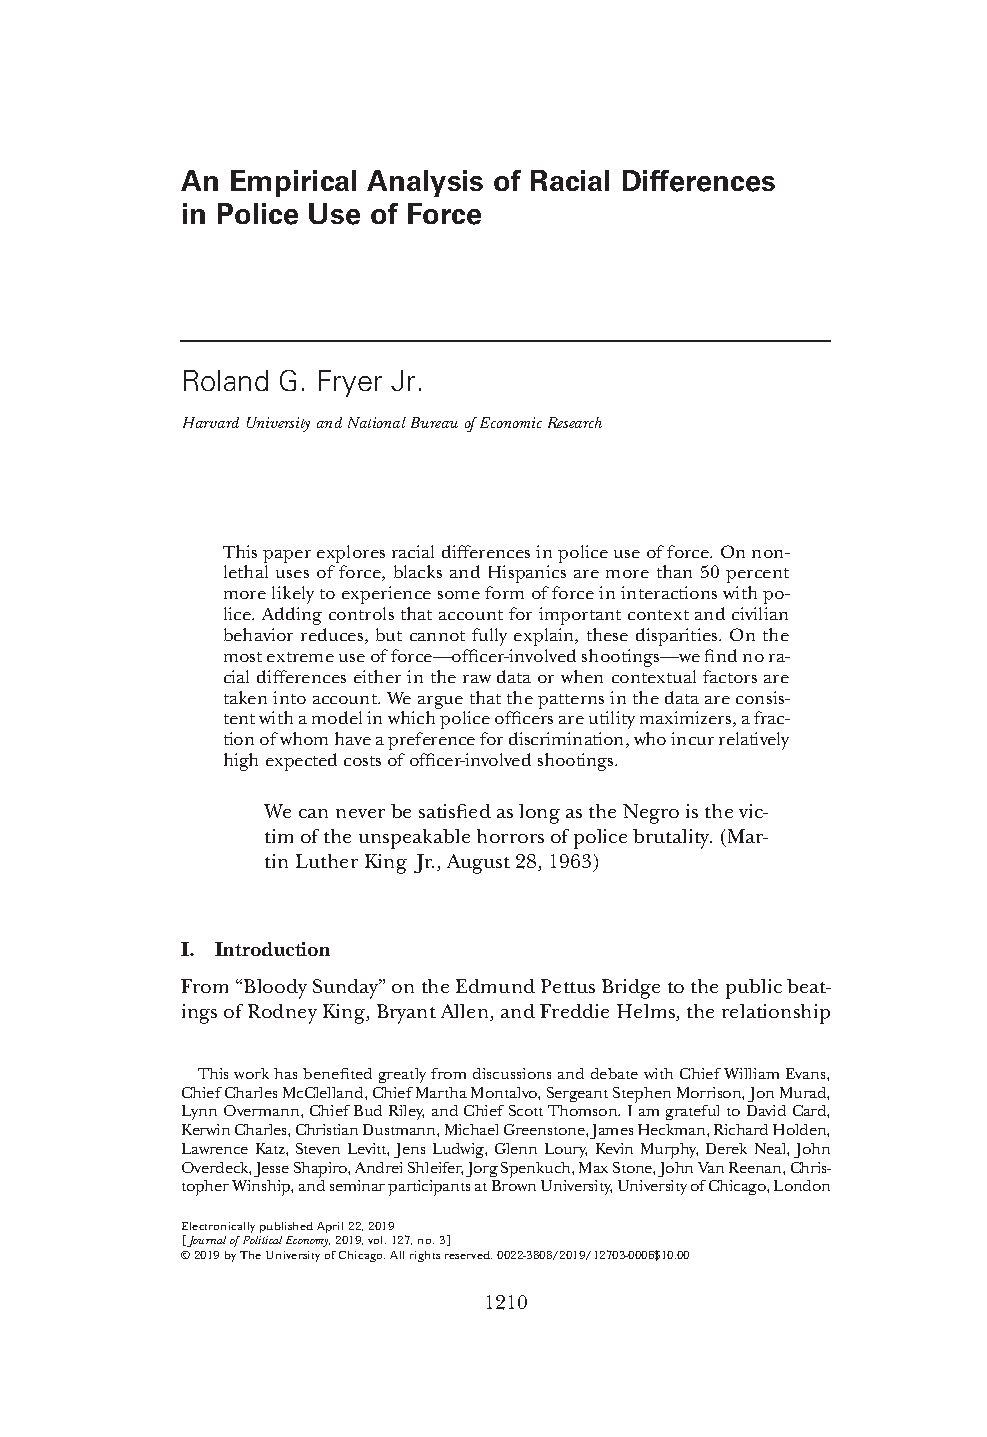
\includegraphics[width = .5\textwidth]{output/fryer_p1}};
    \node<2->[anchor = north east, draw = white, fill = gray, text = black, rounded corners, fill opacity = .2, text opacity = 1, align = left, font = \small] (quote) at (1,1) {It is the most surprising\\result of my career.\\};
    \node<2->[anchor = south east, font = \footnotesize] at (quote.south east) {--- Roland Fryer};
    \node<3->[anchor = east, rotate = 6] at (1,.65) {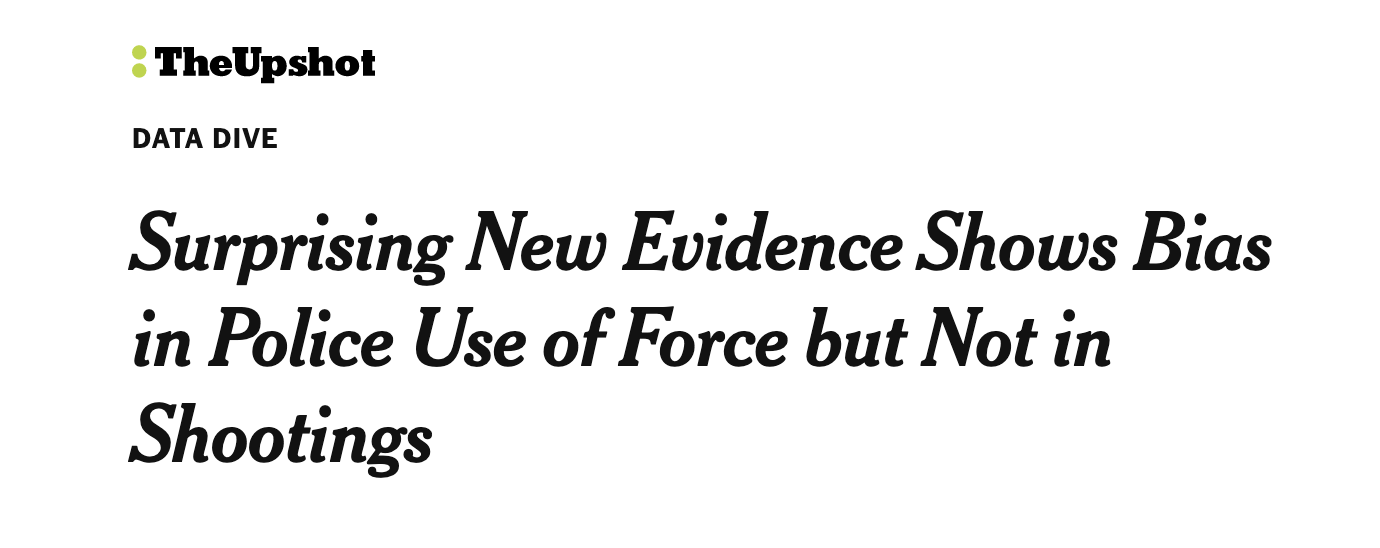
\includegraphics[width = .5\textwidth]{output/fryer_nytimes}};
    \node<4->[anchor = east, rotate = -8] at (1,.3) {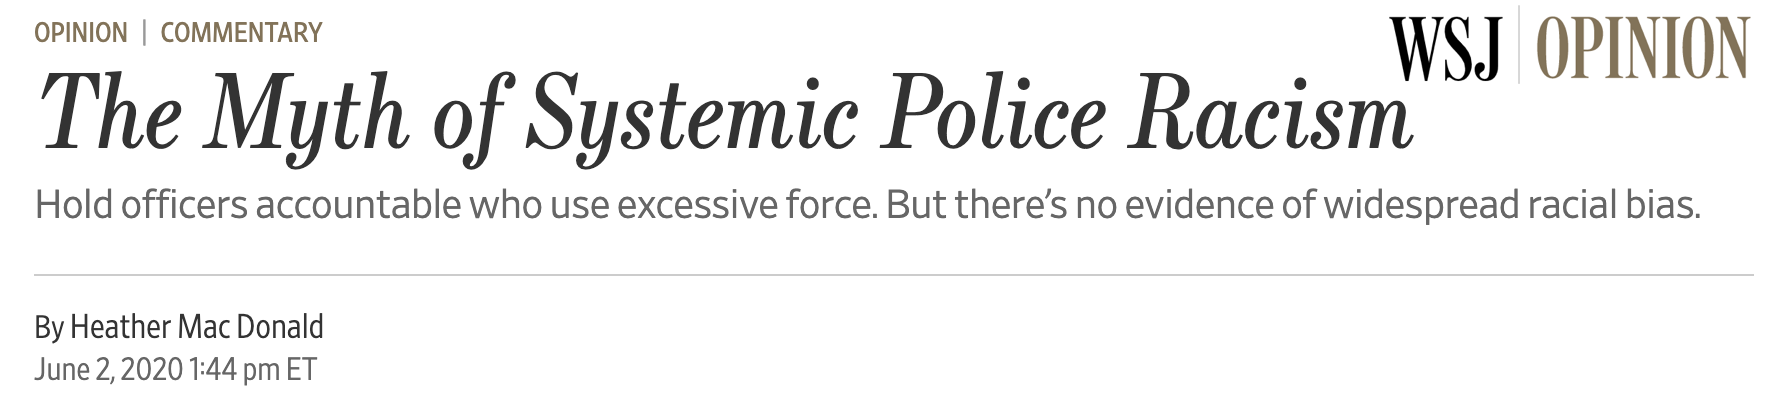
\includegraphics[width = .5\textwidth]{output/fryer_myth_wsj}};
    \node<5->[anchor = east, rotate = 3] at (1,.2) {
\includegraphics[width = .5\textwidth]{output/fryer_guardian}};
    \end{tikzpicture}
    \end{frame}
   
   \begin{frame}
   \headerfigure
    
\begin{tikzpicture}[x = \textwidth, y = .8\textheight]
    \node at (0,0) {};
    \node at (1,1) {};
    % Fryer example
    %\node<3>[anchor = north west, align = left] at (0,.8) {\bgray{Example:} Police-involved shootings by race};
    \node[anchor = north west, font = {\bf\small}, gray, align = left] at (0,.97) {Evidence:};
    \node[anchor = north west, gray, font = {\bf\small}, align = left] (claimLabel) at (0,.82) {Claim:};
    \node[anchor = north west, gray, font = {\bf\small}, align = left] at (0,.72) {Why wrong:};
    \node[anchor = south east, gray, font = \footnotesize] at (1,0) {Fryer 2019. Fuller critique by Knox et al. 2020 and Durlauf and Heckman 2020.};
    \node<2->[anchor = north west, text width = 3in, font = {\small}] at  (.2, .97) {Police use lethal force at the same rate against black and white civilians who are stopped.};
    \node<3->[anchor = north west, text width = 3in, font = {\small}] (claimText) at  (.2,.82) {Police are unbiased};
    \node<10->[anchor = north west, text width = 3in, font = {\small}] (whyText) at (.2,.72) {Causal sample selection. Among those stopped, the white civilians may be more dangerous.};
    %\node<10->[anchor = north west, text width = 3in, font = {\small}] at (whyText.south west) {An unbiased officer might use \textbf{more} force against the white civlians.};
    \node<4-9>[anchor = center, align = center, font = \small] (d) at (.2,.35) {Perceived\\as black};
    \node<4-9>[anchor = center, align=center, font = \small] (y) at (.8,.35) {Lethal force};    
    \draw<4-9>[->, blue, line width = 2pt] (d) to[bend left = 22] (y);
    \node<5-9>[anchor = center, align=center, draw, rounded corners, font = \small] (c) at (.5,.35) {Stopped by\\police};
    \draw<5-9>[->, thick] (d) -- (c);
    \draw<5-9>[->, thick] (c) -- (y);
    \node<6-9>[anchor = center, font = \small] (u) at (.5,.15) {Criminal activity};
    \draw<6-9>[->, thick] (u) -- (c);
    \draw<6-9>[->, thick] (u) -- (y);
    % Visual depiction (will ultimately be its own clicks)
    \draw<7-9>[fill = white, draw = white] (0,.5) rectangle (1,1);
    % Perceived as white
    \node<7-9>[anchor = south, gray] at (.25,.85) {Perceived as \textbf{white}};
    \draw<7-9>[line width = 2pt, gray, line width = 2pt, rounded corners] (.1,.55) rectangle (.4,.85);
    \onslide<7>{
    \node[font = {\tiny\bf}, fill = red, rounded corners, line width = 2pt] at (.3,.8) {\textcolor{white}{Crime}};
    \node[font = {\tiny\bf}, fill = red, rounded corners, line width = 1pt] at (.3,.7) {\textcolor{white}{Crime}};
    \node[font = {\tiny\bf}, fill = gray, rounded corners, line width = 1pt] at (.3,.6) {\textcolor{white}{Safe}};
    \node[font = {\tiny\bf}, fill = gray, rounded corners, line width = 1pt] at (.2,.8) {\textcolor{white}{Safe}};
    \node[font = {\tiny\bf}, fill = gray, rounded corners, line width = 1pt] at (.2,.7) {\textcolor{white}{Safe}};
    \node[font = {\tiny\bf}, fill = gray, rounded corners, line width = 1pt] at (.2,.6) {\textcolor{white}{Safe}};
    }
    \onslide<8-9>{
    \node[font = {\tiny\bf}, draw = black, fill = red, rounded corners, line width = 1.5pt] at (.3,.8) {\textcolor{white}{Crime}};
    \node[font = {\tiny\bf}, draw = black, fill = red, rounded corners, line width = 1.5pt] at (.3,.7) {\textcolor{white}{Crime}};
    \node[opacity = .5, font = {\tiny\bf}, fill = gray, rounded corners, line width = 1.5pt] at (.3,.6) {\textcolor{white}{Safe}};
    \node[opacity = .5, font = {\tiny\bf}, fill = gray, rounded corners, line width = 1.5pt] at (.2,.8) {\textcolor{white}{Safe}};
    \node[opacity = .5, font = {\tiny\bf}, fill = gray, rounded corners, line width = 1.5pt] at (.2,.7) {\textcolor{white}{Safe}};
    \node[opacity = .5, font = {\tiny\bf}, fill = gray, rounded corners, line width = 1.5pt] at (.2,.6) {\textcolor{white}{Safe}};
    }
    % Perceived as black
    \node<7-9>[anchor = south, gray] at (.75,.85) {Perceived as \textbf{black}};
    \draw<7-9>[line width = 2pt, gray, line width = 2pt, rounded corners] (.6,.55) rectangle (.9,.85);
    \onslide<7-8>{
    \node[font = {\tiny\bf}, fill = red, rounded corners, line width = 1pt] at (.8,.8) {\textcolor{white}{Crime}};
    \node[font = {\tiny\bf}, fill = red, rounded corners, line width = 1pt] at (.8,.7) {\textcolor{white}{Crime}};
    \node[font = {\tiny\bf}, fill = gray, rounded corners, line width = 1pt] at (.7,.8) {\textcolor{white}{Safe}};
    \node[font = {\tiny\bf}, fill = gray, rounded corners, line width = 1pt] at (.7,.7) {\textcolor{white}{Safe}};
    \node[font = {\tiny\bf}, fill = gray, rounded corners, line width = 1pt] at (.8,.6) {\textcolor{white}{Safe}};
    \node[font = {\tiny\bf}, fill = gray, rounded corners, line width = 1pt] at (.7,.6) {\textcolor{white}{Safe}};
    }
    \onslide<9>{
    \node[draw = black, font = {\tiny\bf}, fill = red, rounded corners, line width = 1.5pt] at (.8,.8) {\textcolor{white}{Crime}};
    \node[draw = black, font = {\tiny\bf}, fill = red, rounded corners, line width = 1.5pt] at (.8,.7) {\textcolor{white}{Crime}};
    \node[draw = black, font = {\tiny\bf}, fill = gray, rounded corners, line width = 1.5pt] at (.7,.8) {\textcolor{white}{Safe}};
    \node[draw = black, font = {\tiny\bf}, fill = gray, rounded corners, line width = 1.5pt] at (.7,.7) {\textcolor{white}{Safe}};
    \node[opacity = .5, font = {\tiny\bf}, fill = gray, rounded corners, line width = 1.5pt] at (.8,.6) {\textcolor{white}{Safe}};
    \node[opacity = .5, font = {\tiny\bf}, fill = gray, rounded corners, line width = 1.5pt] at (.7,.6) {\textcolor{white}{Safe}};
    }
    % Fryer responds
    \node<11->[anchor = north west, gray, font = {\bf\small}, align = left] at (0,.47) {Fryer\\responds:};
    \draw<12->[thick] (claimLabel.west) -- (claimText.east);
    \node<13->[anchor = north west, draw = white, fill = gray, text = black, rounded corners, fill opacity = .2, text opacity = 1, align = left, font = \small, text width = 3in] at  (.2, .47) {``We use the term `racial differences' 114 times in lieu of the more prescriptive wording---`racial\\discrimination.' We use the phrase `conditional on an interaction' 20 times...I am not sure how many more ways we would have needed to caveat our results to satisfy [the critics].''};
    \end{tikzpicture}
\end{frame}

% ASR REVIEW
\roadmap{.502}{.07}
\roadmap{.435}{.04}

\begin{frame}[t]
\headerfigure
\resizebox{\textwidth}{!}{
    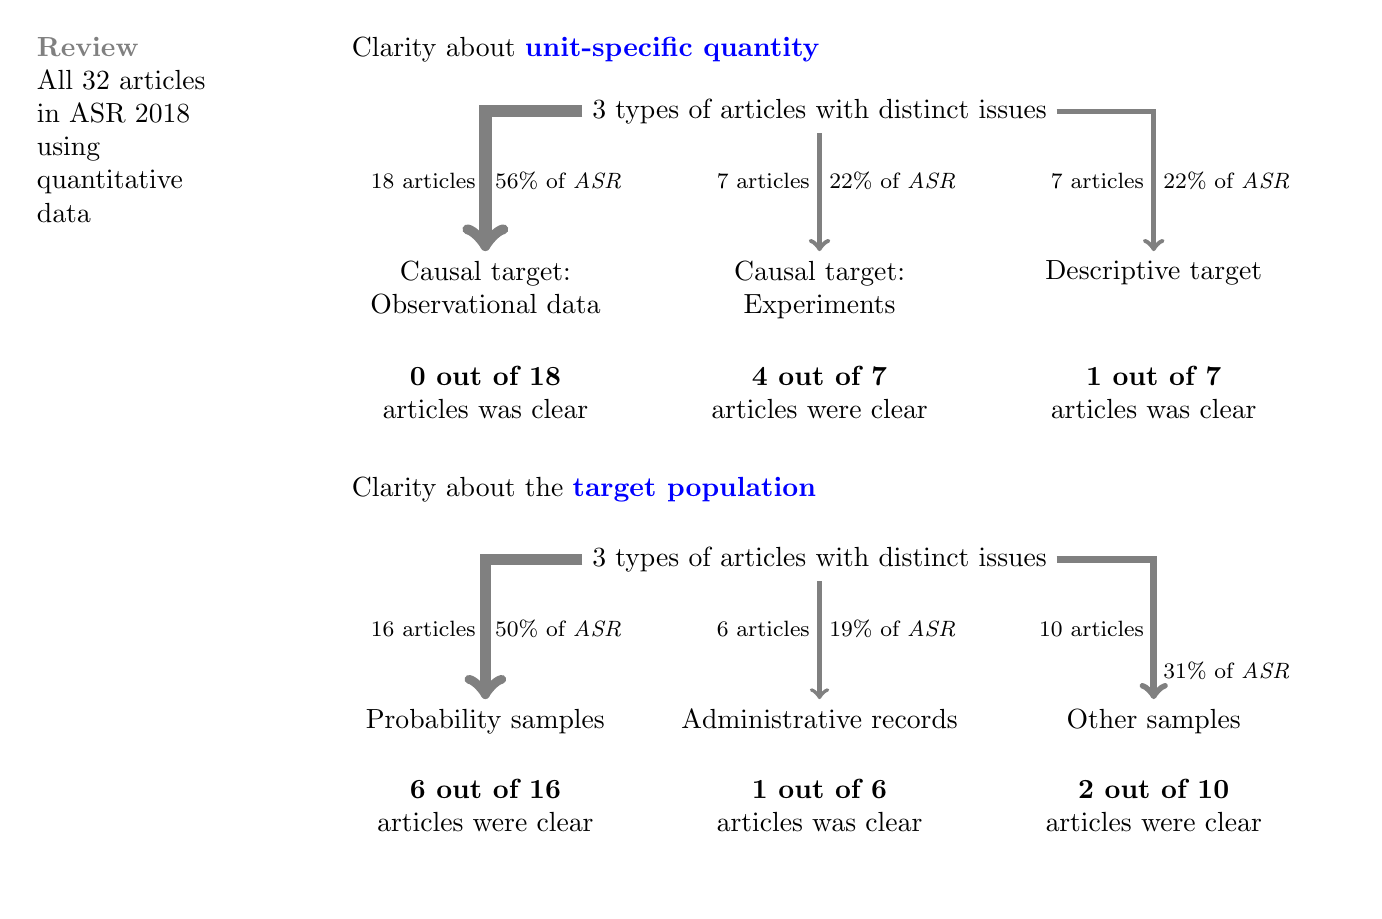
\begin{tikzpicture}[x = \textwidth, y = .7in]
    \node at (1.05,-6.5) {};
    %\draw[line width = 1.5pt] (asr.south west) -- (asr.south east);
    \node[align = left, anchor = north east, text width = 1in] (asr) at (-.1,-.4) {\bgray{Review}\\All 32 articles\\in ASR 2018\\using\\quantitative\\data};
    \node<2->[align = left, anchor = north west] at (0,-.4) {Clarity about \bblue{unit-specific quantity}};
    %\node[align = right, anchor = east] at (1,-.6) {Details in Appendix Table \ref{tab:causal_contrast_overview}};
    \node<2->[align = center] (three) at (.5,-1) {3 types of articles with distinct issues};
    \node<2->[align = center, anchor = north] (causal_observational) at (.15,-2) {Causal target:\\Observational data};
    \node<2->[align = center, anchor = north] (descriptive) at (.85,-2) {Descriptive target};
    \node<2->[align = center, anchor = north] (causal_experiments) at (.5,-2) {Causal target:\\Experiments};
    % Line widths are the percent multiplied by 8
    \draw<2->[->, line width = 4.48pt, gray] (three) -- (.15,-1) -- (causal_observational);
    \draw<2->[->, line width = 1.76pt, gray] (three) -- (causal_experiments);
    \draw<2->[->, line width = 1.76pt, gray] (three) -- (.85,-1) -- (descriptive);
    \node<2->[font = \footnotesize, anchor = east, align = right] at (.15,-1.5) {18 articles};
    \node<2->[font = \footnotesize, anchor = east, align = right] at (.5,-1.5) {7 articles};
    \node<2->[font = \footnotesize, anchor = east, align = right] at (.85,-1.5) {7 articles};
    \node<2->[font = \footnotesize, anchor = west, align = left] at (.15,-1.5) {56\% of \emph{ASR}};
    \node<2->[font = \footnotesize, anchor = west, align = left] at (.5,-1.5) {22\% of \emph{ASR}};
    \node<2->[font = \footnotesize, anchor = west, align = left] at (.85,-1.5) {22\% of \emph{ASR}};
    \node<3->[anchor = north, align = center] at (.15,-2.75) {\textbf{0 out of 18}\\articles was clear};
    \node<3->[anchor = north, align = center] at (.5,-2.75) {\textbf{4 out of 7}\\articles were clear};
    \node<3->[anchor = north, align = center] at (.85,-2.75) {\textbf{1 out of 7}\\articles was clear};
    %%%%%%%%%%%%%%%%%%%%%%%%%%%%%%%%%%
    \node<4->[anchor = west, align = left] at (0,-3.7) {Clarity about the \bblue{target population}};
    \node<4->[align = center] (three_target) at (.5,-4.2) {3 types of articles with distinct issues};
    \node<4->[align = center, anchor = north] (probability_samples) at (.15,-5.2) {Probability samples};
    \node<4->[align = center, anchor = north] (administrative_records) at (.5,-5.2) {Administrative records};
    \node<4->[align = center, anchor = north] (other_samples) at (.85,-5.2) {Other samples};
    \draw<4->[->, line width = 4pt, gray] (three_target) -- (.15,-4.2) -- (probability_samples);
    \draw<4->[->, line width = 1.5pt, gray] (three_target) -- (administrative_records);
    \draw<4->[->, line width = 2.48pt, gray] (three_target) -- (.85,-4.2) -- (other_samples);
    \node<4->[font = \footnotesize, anchor = east, align = right] at (.15,-4.7) {16 articles};
    \node<4->[font = \footnotesize, anchor = east, align = right] at (.5,-4.7) {6 articles};
    \node<4->[font = \footnotesize, anchor = east, align = right] at (.85,-4.7) {10 articles};
    \node<4->[font = \footnotesize, anchor = west, align = left] at (.15,-4.7) {50\% of \emph{ASR}};
    \node<4->[font = \footnotesize, anchor = west, align = left] at (.5,-4.7) {19\% of \emph{ASR}};
    \node<4->[font = \footnotesize, anchor = west, align = left] at (.85,-5) {31\% of \emph{ASR}};
    \node<5->[anchor = north, align = center] at (.15,-5.7) {\textbf{6 out of 16}\\articles were clear};
    \node<5->[anchor = north, align = center] at (.5,-5.7) {\textbf{1 out of 6}\\articles was clear};
    \node<5->[anchor = north, align = center] at (.85,-5.7) {\textbf{2 out of 10}\\articles were clear};
    %\node<12->[align = left, fill = white, draw = gray, line width = 2pt, rounded corners] at (.5,-3.5) {Lack of clarity\\--- Not clear what a study has shown\\--- How evidence informs theory is vague\\--- Not clear why results differ across studies};
    %\node<6->[align = left, anchor = north west, text width = 1.1in] (consequences) at (asr.south west) {\textcolor{white}{filler}\\\textcolor{white}{filler}\\\bgray{Confusion}\\arises about\\\only<7->{theory,}\only<8->{ methods,\\}\only<9->{ and conflicting\\studies.}};
    \end{tikzpicture}}
    \end{frame}

% REPLICATIONS
\roadmap{.435}{.04}
\roadmap{.365}{.04}

% PAL AND WALDFOGEL
\begin{frame}[t]
\headerfigure \vskip .6in
\bgray{Replication 1}
\begin{itemize}
\item Define a tricky theoretical estimand
\item Reveal overlooked identification assumptions
\item Show the mechanics of estimation by machine learning
\end{itemize}
\end{frame}
\begin{frame}[t]
\only<1>{\headerfigure}
\only<2-9>{\headerfigureset}
\only<10-18>{\headerfigurelink}
\only<19->{\headerfigurelearn}
\begin{tikzpicture}[x = \textwidth, y = .8\textheight]
\node at (0,0) {};
\node at (1,1) {};
\node<1-9>[anchor = north west] at (0,1) {Pal and Waldfogel (2016) estimate the family gap in pay.};
\node<2-9>[anchor = north west] (descriptive) at (0,.9) {Is the theoretical estimand descriptive?};
\node<3-4>[anchor = north, align = center] at (.5, .8) {``the differential in hourly wages\\between women with children\\and women without children''};
%\node<4->[anchor = north west, align = left] (descriptive) at (.05,.8) {Is it descriptive?};% They estimate ``the differential in hourly wages\\between women with children and women without children.''};
\node<4>[anchor = south, font = {\gray\footnotesize}] (mothers) at (.25, 0) {of \bblue{mothers}};
\node<4>[anchor = south, font = {\gray\footnotesize}] (nonmothers) at (.75, 0) {of \bred{non-mothers}};
\node<4>[anchor = south] at (.25,.03) {\estimandFigureBottomCaptionCustom{$Y_i$}{\footnotesize}{8pt}{1}{1}};
\node<4>[anchor = south] at (.75,.03) {\estimandFigureBottomCaptionCustomDiamond{$Y_i$}{\footnotesize}{6pt}{1}{1}};
\node<5-9>[anchor = north west] at (descriptive.north east) {Is it causal?};
\node<6-7>[anchor = north] at (.5, .8) {``causal estimation techniques''};
\node<7-8>[anchor = south] at (.5,0) {
	\begin{tikzpicture}[x = 1.7\textwidth, y = 1.4\textheight, every node/.style={anchor = center}]
	\node[circle, fill = lightgray, draw = lightgray, inner sep = 22pt] (point1) at (.15,.47) {};
	\node[gray, font = \footnotesize, align = center, anchor = north] (usqNote) at (point1.south) {A \bgray{unit-specific}\\\bgray{quantity}};
	\node[circle, fill = lightgray, draw = lightgray, inner sep = 22pt] (point2) at (.3,.5) {};
	\node[circle, fill = lightgray, draw = lightgray, inner sep = 22pt] (point3) at (.41,.39) {};
	\draw[line width = 2pt, gray, rounded corners] (.05,.3) rectangle (.5,.6);
	\node[gray, font = \footnotesize, align = center, anchor = north] at (.275,.3) {Averaged over a\\\bgray{target population}\\of \bgray{mothers}};
	\node[font = \tiny, align = left] at (point1) {$Y_i\left(\begin{matrix}\text{Mother}\end{matrix}\right)$\\-$Y_i\left(\begin{matrix}\text{Non-mother}\end{matrix}\right)$};
	\node[font = \tiny, align = left] at (point2) {$Y_i\left(\begin{matrix}\text{Mother}\end{matrix}\right)$\\-$Y_i\left(\begin{matrix}\text{Non-mother}\end{matrix}\right)$};
	\node[font = \tiny, align = left] at (point3) {$Y_i\left(\begin{matrix}\text{Mother}\end{matrix}\right)$\\-$Y_i\left(\begin{matrix}\text{Non-mother}\end{matrix}\right)$};
	\end{tikzpicture}
};
\node<8-9>[anchor = north west] at (0, .8) {Added complexity: Wages are undefined for the non-employed.};
\node<9>[anchor = south] at (.5,0) {
	\begin{tikzpicture}[x = 1.7\textwidth, y = 1.4\textheight, every node/.style={anchor = center}]
	\node[circle, fill = lightgray, draw = lightgray, inner sep = 22pt] (point1) at (.15,.47) {};
	\node[gray, font = \footnotesize, align = center, anchor = north] (usqNote) at (point1.south) {A \bgray{unit-specific}\\\bgray{quantity}};
	\node[circle, fill = lightgray, draw = lightgray, inner sep = 22pt] (point2) at (.3,.5) {};
	\node[circle, fill = lightgray, draw = lightgray, inner sep = 22pt] (point3) at (.41,.39) {};
	\draw[line width = 2pt, gray, rounded corners] (.05,.3) rectangle (.5,.6);
	\node[gray, font = \footnotesize, align = center, anchor = north] at (.275,.3) {Averaged over a\\\bgray{target population}\\of \bgray{mothers}};
	\node[font = \tiny, align = left] at (point1) {$Y_i\left(\begin{matrix}\text{Mother}\\\text{Employed}\end{matrix}\right)$\\-$Y_i\left(\begin{matrix}\text{Non-mother}\\\text{Employed}\end{matrix}\right)$};
	\node[font = \tiny, align = left] at (point2) {$Y_i\left(\begin{matrix}\text{Mother}\\\text{Employed}\end{matrix}\right)$\\-$Y_i\left(\begin{matrix}\text{Non-mother}\\\text{Employed}\end{matrix}\right)$};
	\node[font = \tiny, align = left] at (point3) {$Y_i\left(\begin{matrix}\text{Mother}\\\text{Employed}\end{matrix}\right)$\\-$Y_i\left(\begin{matrix}\text{Non-mother}\\\text{Employed}\end{matrix}\right)$};
	\end{tikzpicture}
};
% Move the USQ up
    \node<10-14>[anchor = north west] at (0, 1) {\bgray{Unit-specific quantity:} $Y_i\left(\begin{matrix}\text{Mother,}\\\text{Employed}\end{matrix}\right) - Y_i\left(\begin{matrix}\text{Non-mother,}\\\text{Employed}\end{matrix}\right)$};
    \node<11-18>[anchor = east, align = left, font = \footnotesize, gray] at (.35,.2) {Education\\Married\\Race\\Age};
    \node<11-18>[font = \small] (x) at (.35,.2) {$\vec{X}$};
    \node<11-18>[font = \small] (motherhood) at (.5,.2) {Motherhood};
    \node<11-18>[font = \small, align = center] (employment) at (.65,.3) {Employed};
    \node<11-18>[font = \small, align = center] (earnings) at (.8,.2) {Wage};
    \node<12-18>[font = \small, align = center, red] (u1) at (.5,.07) {$U_1$};
    \node<13-18>[font = \small, align = center, red] (u2) at (.8,.3) {$U_2$};
    \draw<11-18>[->, thick] (x) -- (motherhood);
    \draw<11-18>[->, thick] (x) to[out = 45, in = 180] (employment);
    \draw<11-18>[->, thick] (x) to[out = 300, in = 240] (earnings);
    \draw<11-18>[->, thick] (motherhood) -- (employment);
    \draw<11-18>[->, line width = 2pt, blue] (motherhood) -- (earnings);
    \draw<11-18>[->, thick] (employment) -- (earnings);
    \draw<12-18>[->, thick, red, dashed] (u1) -- (motherhood);
    \draw<12-18>[->, thick, red, dashed] (u1) -- (earnings);
    \draw<13-18>[->, thick, red, dashed] (u2) -- (employment);
    \draw<13-18>[->, thick, red, dashed] (u2) -- (earnings);
\node<15-18>[anchor = east, font = \scriptsize] at (.46,.9) {$\E\left(Y_i\left(\begin{matrix}\text{Mother},\\\text{Employed}\end{matrix}\right)\hspace{2pt}\Bigg\vert\hspace{2pt} \vec{X} = \vec{x}_i\right)$};
\node<17->[anchor = west, font = \scriptsize] at (.5,.9) {$\E\left(Y_i\hspace{2pt}\Bigg\vert\hspace{2pt} \begin{matrix}\text{Motherhood} &=&\text{Mother},\\\text{Employment} &=& \text{Employed},\\\text{Covariates }\vec{X} &=& \text{Observed }\vec{x}_i\end{matrix}\right)$};
\node<17> (equals) at (.48,.9) {$?$};
% Visually depict the potential outcomes
\node<14-18>[anchor = south, font = \scriptsize, align = center] at (.23,.75) {\bgray{Potential} outcomes};
\draw<14-18>[gray, line width = 2pt, rounded corners] (.02,.4) rectangle (.44,.75);
\node<14-18>[gray, font = \scriptsize, anchor = south west, align = left] (focus) at (.02,.2) {Focus on\\one $\vec{X} = \vec{x}_i$};
\draw<14-18>[->, gray, line width = 1.2pt] (focus) to[bend left] (.1,.38);
\node<14-15>[font = \tiny, rounded corners, fill = lightgray, inner sep = 2pt] at (.12,.67) {$Y_i\left(\begin{matrix}\text{Mother},\\\text{Employed}\end{matrix}\right)$};
\node<16-18>[font = \tiny, opacity = .4, rounded corners, fill = lightgray, inner sep = 1pt] at (.12,.67) {$Y_i\left(\begin{matrix}\text{Mother},\\\text{Employed}\end{matrix}\right)$};
\node<14-18>[font = \tiny, rounded corners, fill = lightgray, inner sep = 2pt] at (.25,.58) {$Y_i\left(\begin{matrix}\text{Mother},\\\text{Employed}\end{matrix}\right)$};
\node<14-18>[font = \tiny, rounded corners, fill = lightgray, inner sep = 2pt] at (.33,.68) {$Y_i\left(\begin{matrix}\text{Mother},\\\text{Employed}\end{matrix}\right)$};
\node<14-18>[gray, font = \scriptsize, anchor = south west, align = left] at (.02,.4) {All women\\with a high school degree,\\married, white, age 30};
% Visually depict the realized
\draw<17->[gray, line width = 2pt, rounded corners] (.52,.4) rectangle (.94,.75);
\node<17->[font = \scriptsize, rounded corners, fill = lightgray, inner sep = 4pt] at (.75,.58) {$Y_i$};
\node<17->[font = \scriptsize, rounded corners, fill = lightgray, inner sep = 4pt] at (.83,.68) {$Y_i$};
\node<17->[gray, font = \scriptsize, anchor = south west, align = left] at (.52,.4) {\textbf{Employed mothers}\\with a high school degree,\\married, white, age 30};
\node<17->[anchor = south, font = \scriptsize, align = center] at (.73,.75) {\bgray{Realized} outcomes};
%\node<14-16>[anchor = north, font = \scriptsize, align = center] at (.23,.2) {The \bgray{theoretical estimand}\\is the population average\\of these.};
%\node<15->[anchor = north, font = \scriptsize, align = center] at (.75,.2) {The \bgray{empirical estimand}\\is the population average\\of these.};
\node<18> (equals) at (.48,.9) {$=$};
\node<18>[font = \scriptsize, align = center, anchor = north] (dag) at (.48, .87) {By the\\DAG};
%\draw<16>[->, thick] (dag) -- (.43,.75);
%\draw<16>[->, thick] (dag) -- (.53,.75);
\node<20->[align = center] (mlHelps) at (.185,.9) {This can be estimated\\by \bgray{machine learning}!};
\draw<20->[->, gray, line width = 2pt] (mlHelps) -- (.5, .9);
\draw<20->[line width = 1.5pt, gray, line cap = rounded] (.06,.83) -- (.34, .83); % underlines ML
\draw<21->[->, line width = 1.5pt, gray] (.2,.83) -- (.2,.77);  % ML to prediction algorithm
\node<21->[font = \footnotesize, align = center] at (.2,.72) {Any prediction algorithm\\that minimizes squared errors};
\node<22->[font = \scriptsize, align = center, anchor = north] at (.2,.55) {Generalized\\Additive\\Model};
\node<23->[font = \scriptsize, align = center, anchor = north] at (.33,.55) {Random\\Forest};
\node<24->[font = \scriptsize, align = center, anchor = north] at (.07,.55) {Ordinary\\Least\\Squares};
\draw<22->[->, line width = 1.5pt, gray] (.2,.65) -- (.2,.55);
\draw<23->[->, line width = 1.5pt, gray] (.23,.65) -- (.28,.55);
\draw<24->[->, line width = 1.5pt, gray] (.17,.65) -- (.12,.55);
\end{tikzpicture}
\end{frame}

\begin{frame}[t]
\headerfigurelearn
\begin{tikzpicture}[x = \textwidth, y = .8\textheight]
\node at (0,0) {};
\node at (1,1) {};
\node[anchor = north west] at (0,1) {Mechanics: How \bblue{predictive algorithms} estimate the \bblue{estimand}};å
\node<2->[anchor = north west] at (0,.9) {1) Learn an algorithm to predict the outcome};
\node<3->[anchor = north west] at (0,.8) {2) Predict for every unit at each treatment value};
%%%%%%%%%%
\node<4>[anchor = east] at (.32,.6) {$\hat{Y}_i\left(\begin{matrix}\texttt{Mother},\\\texttt{Employed}\end{matrix}\right)$}; 
\node<4> at (.34,.6) {$=$};
\node<3-4>[anchor = west] at (.36,.6) {$\hat\E\left(Y_i\hspace{2pt}\Bigg\vert\hspace{2pt} \begin{matrix}\text{Motherhood} &=&\texttt{Mother},\\\text{Employment} &=& \texttt{Employed},\\\text{Covariates }\vec{X} &=& \texttt{Observed }\vec{x}_i\end{matrix}\right)$};
%%%%%%%%%%
\node<5->[anchor = east] at (.32,.6) {$\hat{Y}_i\left(\begin{matrix}\texttt{Non-mother},\\\texttt{Employed}\end{matrix}\right)$}; 
\node<5-> at (.34,.6) {$=$};
\node<5->[anchor = west] at (.36,.6) {$\hat\E\left(Y_i\hspace{2pt}\Bigg\vert\hspace{2pt} \begin{matrix}\text{Motherhood} &=&\texttt{Non-mother},\\\text{Employment} &=& \texttt{Employed},\\\text{Covariates }\vec{X} &=& \texttt{Observed }\vec{x}_i\end{matrix}\right)$};
%%%%%%%%%%
\node<7->[anchor = north west] at (0,.45) {3) Average over the target population};
\node<6-> at (.5,.3) {$\phantom{\frac{1}{n}\sum_{i=1}^n\Bigg(}\hat{Y}_i\left(\begin{matrix}\texttt{Mother},\\\texttt{Employed}\end{matrix}\right) - \hat{Y}_i\left(\begin{matrix}\texttt{Non-mother},\\\texttt{Employed}\end{matrix}\right)\phantom{\Bigg)}$};
\node<7-> at (.5,.3) {$\frac{1}{n}\sum_{i=1}^n\Bigg(\phantom{\hat{Y}_i\left(\begin{matrix}\texttt{Mother},\\\texttt{Employed}\end{matrix}\right) - \hat{Y}_i\left(\begin{matrix}\texttt{Non-mother},\\\texttt{Employed}\end{matrix}\right)}\Bigg)$};
%%%%%%%%%%
\node<8->[anchor = south east, align = right, font = \footnotesize, gray] at (1,.03) {Hahn, 1998\\Abadie \& Imbens 2006\\Also called the parametric $g$-formula in biostatistics, Hernán \& Robins 2020};
\node<8->[anchor = north west, align = left] at (0,.2) {This is called an \bblue{imputation estimator}};
\end{tikzpicture}
\end{frame}

\begin{frame}[t]
\headerfigurelearn
\begin{tikzpicture}[x = \textwidth, y = .8\textheight]
\node at (0,0) {};
\node at (1,1) {};
\node[anchor = west, font = \large] at (0,.95) {Choose an algorithm by \bblue{predictive performance}};
\node[anchor = north west] at (0,.85) {\bgray{Outcome}};
\node[anchor = north west] at (.2,.85) {Log hourly wage};
\node[anchor = north west] at (0,.75) {\bgray{Predictors}};
\node[anchor = north west] at (.2,.75) {Motherhood, age, race, education, marital status};
\node<2->[anchor = north west] at (0,.65) {\bgray{Candidate algorithms}};
\node<2->[anchor = north west, font = \footnotesize, align = center] at (0,.55) {Least flexible};
\node<2->[anchor = north west, font = \footnotesize, align = center] at (0,.27) {Most flexible};
\node<3->[anchor = north west, font = \small] at (.25,.55) {OLS with a quadratic for age};
\node<4->[anchor = north west, font = \small] at (.25,.48) {+ Interaction between age and motherhood};
\node<5->[anchor = north west, font = \small] at (.25,.41) {+ Allow a smooth curve for age rather than  quadratic};
\node<6->[anchor = north west, font = \small] at (.25,.34) {+ Include each age as a separate indicator variable};
\node<7->[anchor = north west, font = \small] at (.25,.27) {+ Include all interactions among all predictors};
\node<10->[anchor = north west, blue, font = \footnotesize, align = center] at (0,.48) {Best predictions};
\node<8->[anchor = north west] at (0,.15) {Choices about \bblue{functional form}};
\node<9->[anchor = north west] at (0,.15) {Choices about \bblue{functional form} are best decided by the data};
\end{tikzpicture}
\end{frame}

\begin{frame}[t]
\headerfigure
\begin{tikzpicture}[x = \textwidth, y = .8\textheight]
\node at (0,0) {};
\node at (1,1) {};
\node[anchor = north west, font = \large] at (0,1) {Our framework partitions research choices};
\node[anchor = north west] at (0,.9) {Some choices must be \bblue{theory-driven}};
\node[anchor = north west, font = \small] at (0.03,.82) {--- What question is important?};
\node[anchor = north west, font = \small] at (0.03,.74) {--- What variables should I adjust?};
\node[anchor = north east, font = \small, gray] at (1,.82) {theoretical estimand};
\node[anchor = north east, font = \small, gray] at (1,.74) {empirical estimand};
\node[anchor = north west] at (0,.64) {Some choices can be \bblue{data-driven}};
\node[anchor = north west, font = \small] at (0.03,.56) {--- Do I include a squared term?};
\node[anchor = north west, font = \small] at (0.03,.48) {--- Do I need an interaction?};
\node[anchor = north east, font = \small, gray] at (1,.56) {estimation strategy};
\end{tikzpicture}
\end{frame}

% BUCHMANN AND DIPRETE
\begin{frame}[t]
\headerfigure \vskip .6in
\bgray{Replication 2} \vskip .2in
Coefficient-based reasoning hampers understanding
\end{frame}

{
\setbeamertemplate{footline}[text line]{%
\parbox{\linewidth}{}}
\begin{frame}
\centering
\begin{tikzpicture}[x = \textwidth, y = \textheight]
%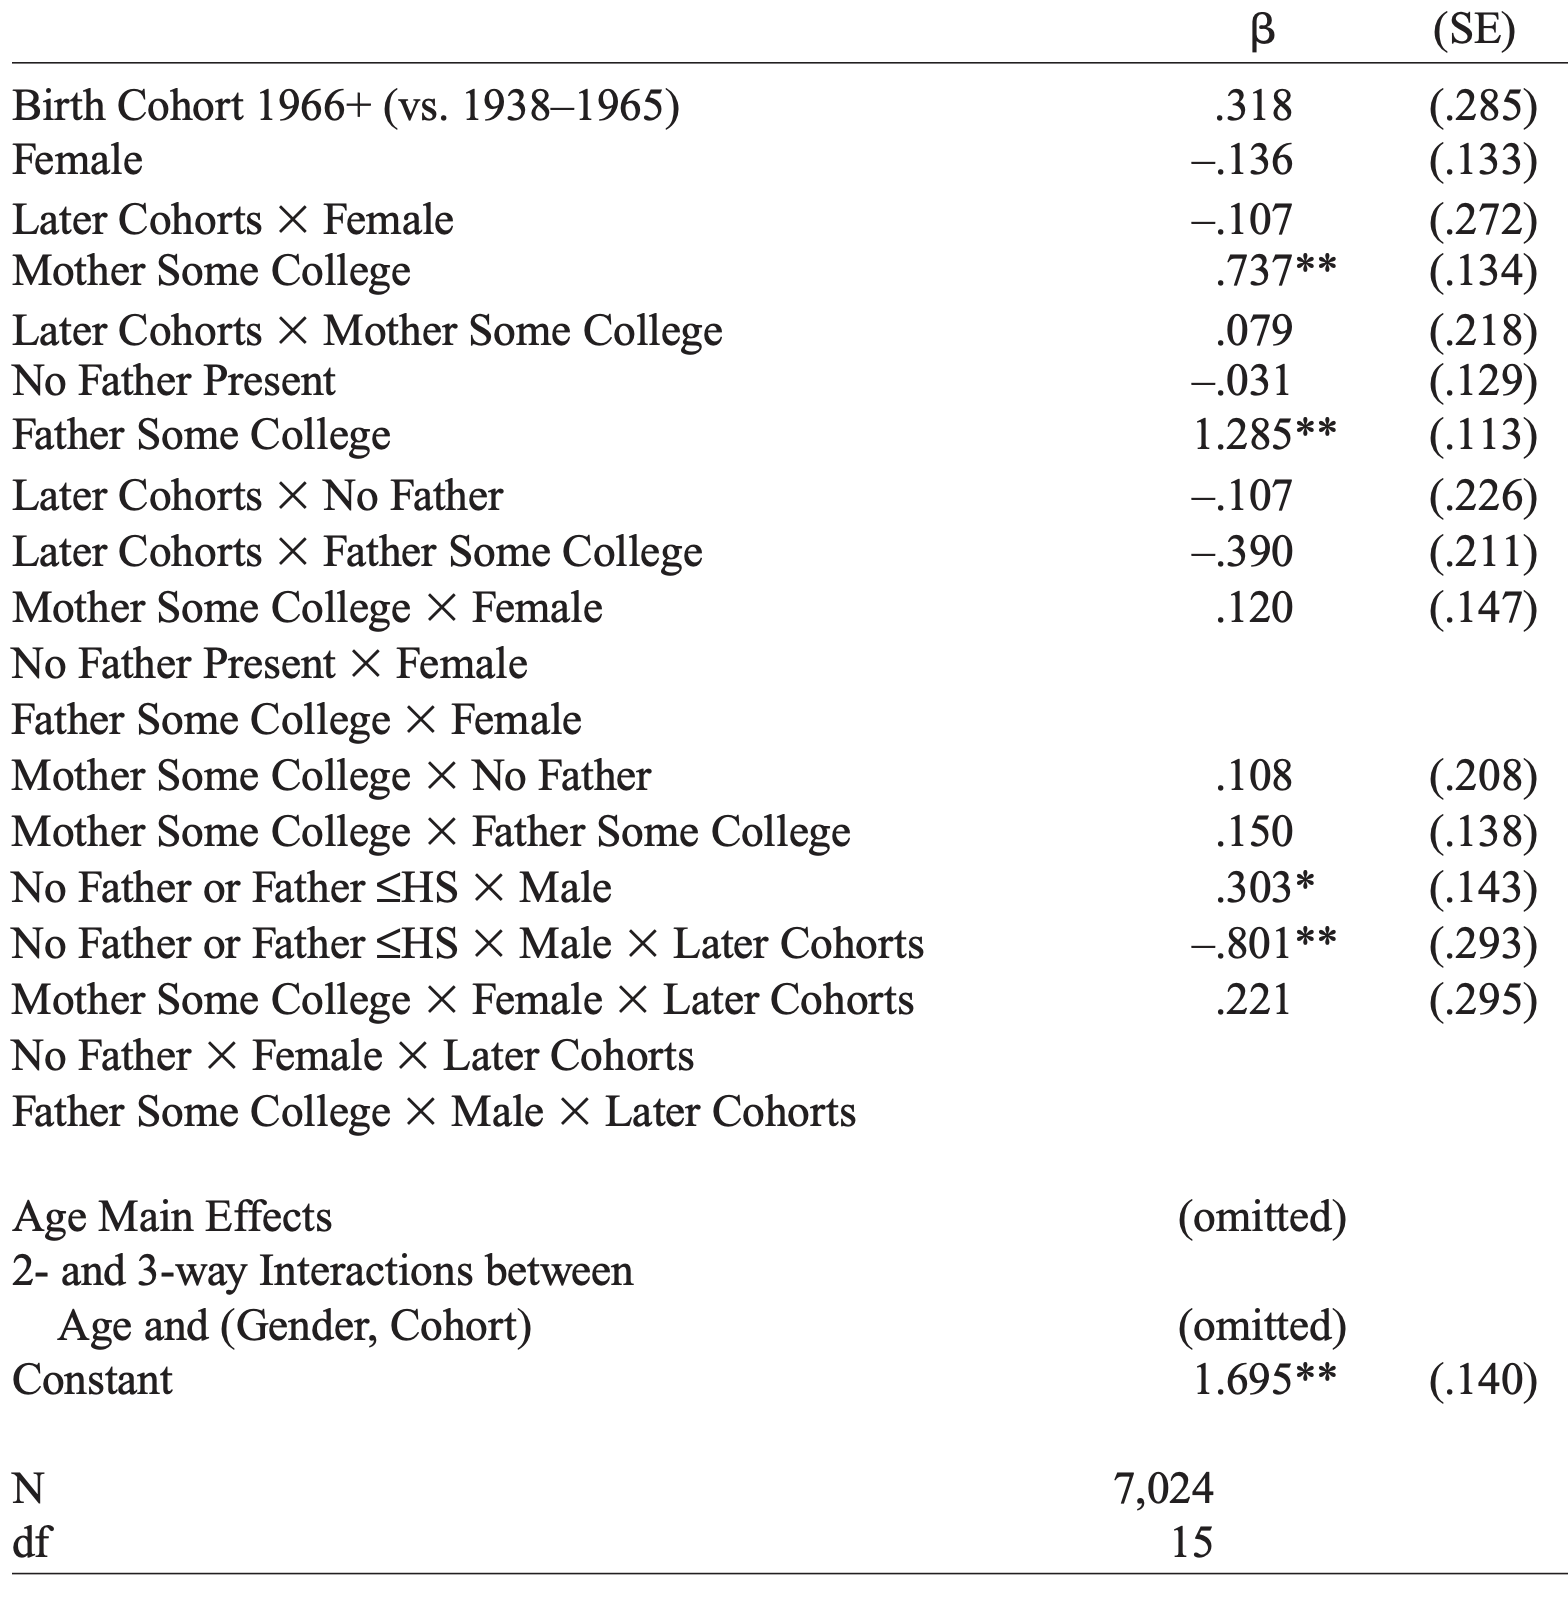
\includegraphics[height = \textheight]{output/buchmann_diprete_table}
\node[line width = 2pt, white] at (1.12,.39) {};
\node[line width = 2pt, white] at (.05,.39) {};
\node[anchor = north east] at (1,1) {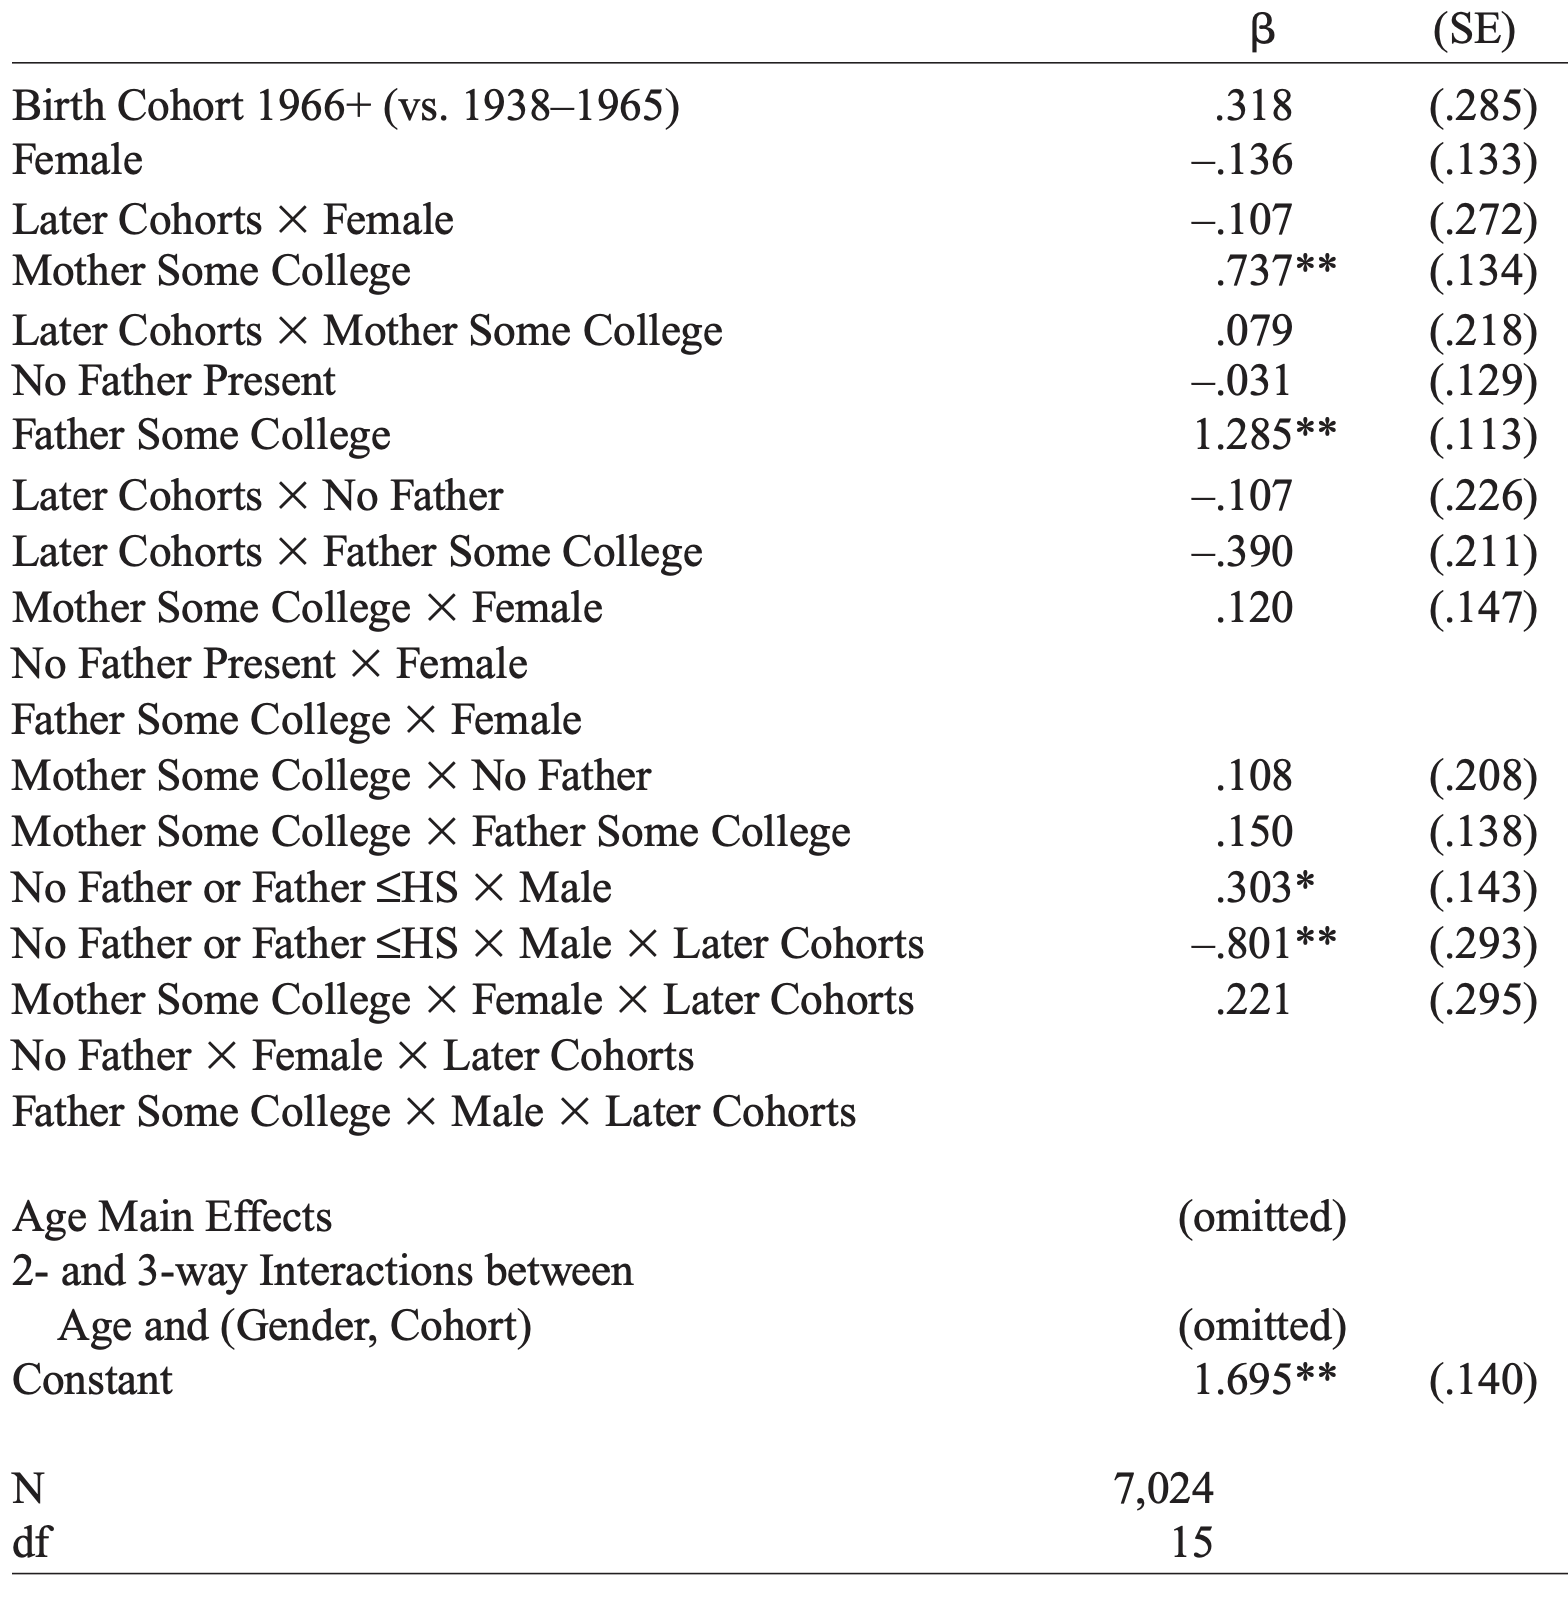
\includegraphics[height = \textheight]{output/buchmann_diprete_table}};
\draw<2>[->, line width = 2pt, blue] (0.06,.394) -- (.11,.394);
\draw<2>[->, line width = 2pt, blue] (.7,.394) -- (.75,.394);
%\node[anchor = north west, align = left] (logit) at (-.1,1) {Logit\\predicting\\college\\completion};
%\node[anchor = north west, align = left, font = \footnotesize, gray] at (logit.south west) {Buchmann\\and\\DiPrete\\2006};
\end{tikzpicture}
\end{frame}
}

\begin{frame}[t]
\headerfigure \vskip .1in
%Example: Coefficients needlessly complicate descriptive estimands\vskip .1in
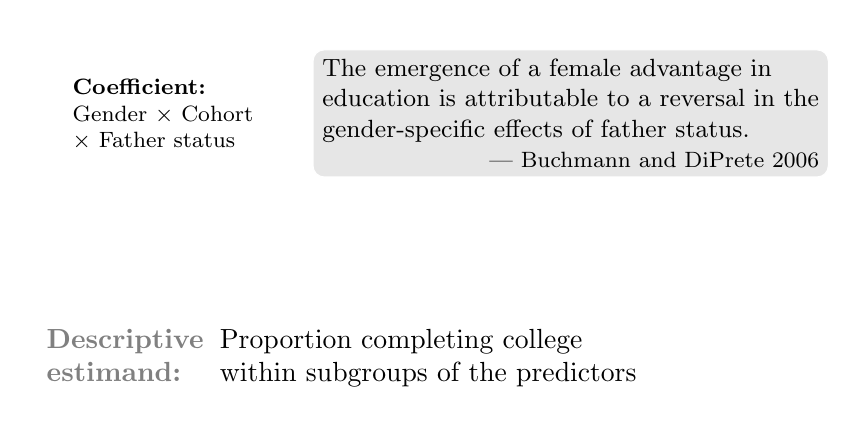
\begin{tikzpicture}
\node at (-3.5,.8) {};
\node<1->[anchor = north west, align = left, font = \small] at (0,1.91) {};
\node<1->[anchor = south west, draw = white, fill = gray, text = black, rounded corners, fill opacity = .2, text opacity = 1, align = left, font = \small] (quote) at (0,0) {The emergence of a female advantage in\\education is attributable to a reversal in the\\gender-specific effects of father status.\\};
\node<1->[anchor = south east, font = \footnotesize] at (quote.south east) {--- Buchmann and DiPrete 2006};
\node<1->[font = \footnotesize, align = left] (interaction) at (-1.9, .8) {\textbf{Coefficient:}\\Gender $\times$ Cohort\\$\times$ Father status};
%\node<2-3>[anchor = north west] at (-3.5, -.6) {\bgray{Outcome:}};
%\node<2-3>[anchor = north west] at (-1.3, -.6) {College completion};
%\node<2-3>[anchor = north west] at (-3.5, -1.1) {\bgray{Predictors:}};
%\node<2-3>[anchor = north west] at (-1.3, -1.1) {Gender, cohort, mother's education, father's education};
\node<2>[anchor = north west, align = left] at (-3.5, -1.8) {\bgray{Descriptive}\\\bgray{estimand:}};
\node<2>[anchor = north west, align = left] at (-1.3, -1.8) {Proportion completing college\\within subgroups of the predictors};
%\draw<2->[->, thick] (interaction) -- (-.2,.8);
\end{tikzpicture}
%Buchmann and DiPrete (2006): 
\resizebox{\textwidth}{!}{\begin{tikzpicture}[x = 6.5in, y = 1in]
\node<3>[anchor = north west] (A_plot) at (0,-.5) {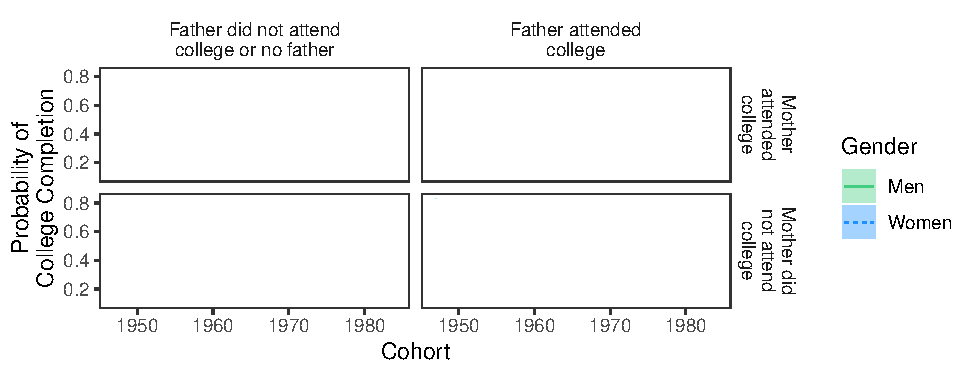
\includegraphics{output/gss_fourPanel_set_stage}};
\node<4->[anchor = north west] (A_plot) at (0,-.5) {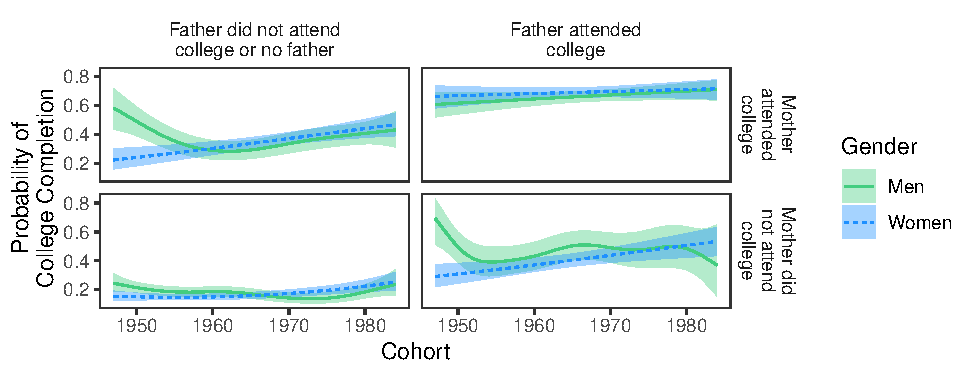
\includegraphics{output/gss_fourPanel_slideFigure}};
% Annotations on high completion group
%\draw[->, seagreen, thick] (.49,-1.45) to[bend left] (.47,-1.33);
%\draw[->, seagreen, thick] (.74,-1.4) to[bend right] (.75,-1.25);
% Annotations on groups with some disadvantage
\onslide<5->{
\draw[->, seagreen, thick] (.22,-2) to[bend left] (.13,-1.4);
\draw[->, seagreen, thick] (.22,-2.1) to[bend right] (.13,-2.35);
\draw[->, seagreen, thick] (.35,-2) -- (.45,-2);
\node[seagreen, fill = white, align = center, rounded corners, draw = seagreen] at (.285, -2.05) {Unusually high\\completion\\among men};
}
\end{tikzpicture}}
\onslide<6->{\bgray{Alternate theory}: The Vietnam War}
\end{frame}

% GAP-CLOSING
\roadmap{.365}{.04}
\roadmap{.295}{.04}

{ 
\setbeamertemplate{footline}[text line]{}
\begin{frame}
\begin{tikzpicture}[x = \textwidth, y = \textheight]
\node at (0,0) {};
\node at (1,1) {};
\node<2->[anchor = north west] at (0,.9) {\bgray{Standard practice:} Report the coefficient on race, gender, or class.};
\node<3->[anchor = north west] at (0,.82) {But is ``treatment'' the right role for these complex constructs?};
\node<4->[align = left, font = \small, anchor = west] (constrain) at (.6,.6) {Familiar\\methods};
\node<4->[align = right, font = \small, anchor = east] (questions) at (.4,.6) {Question\\we ask};
\draw<4->[->, red, line width = 2pt] (constrain) -- node[midway, above, font  = {\bf\footnotesize}] {constrain} (questions);
\node<5->[align = right, font = \small, anchor = east] (theory) at (.4,.45) {Theoretical\\questions};
\node<5->[align = left, font = \small, anchor = west] (data) at (.6,.45) {Things we\\do to data};
\draw<5->[->, seagreen, line width = 2pt] (theory) -- node[midway, above, font  = {\bf\footnotesize}] {motivate} (data);
\node[anchor = south west, font = \small, gray, align = left] at (0,.05) {\textbf{The Gap-Closing Estimand:}\\A Causal Approach to Study Interventions\\That Close Disparities Across Social Categories};
\node[anchor = south east, font = \small, gray, align = right] at (1,.05) {Lundberg, Ian\\Working paper\\On \bref{https://doi.org/10.31235/osf.io/gx4y3}{SocArxiv}};
\end{tikzpicture}
\end{frame}
}

%\node[anchor = north east, align = right, font = \scriptsize, gray] at (1,1) {Lundberg, Ian. Working paper.\\
%The gap-closing estimand:\\
%A causal approach to study\\
%interventions that close\\
%disparities across social\\
%categories};

{ 
\setbeamertemplate{footline}[text line]{}
% Lundberg, Ian. ``The Gap-Closing Estimand: A Causal Approach to Study Interventions that Close Disparities across Social Categories
\begin{frame}
\begin{tikzpicture}[x = \textwidth, y = \textheight]
\node at (0,0) {};
\node at (1,1) {};
\node[align = right, anchor = east] at (1,.75) {Collections of units};
% Denote types of variables
\node<1->[align = left, anchor = west, font = \small] at (0,.75) {Race\\Class Origin\\Gender};
% CATEGORIES
\node[font = \footnotesize, align = center, anchor = south] (category1) at (.3,.85) {Gap-Defining\\Category\\$X = x$};
\node[font = \footnotesize, align = center, anchor = south] (category2) at (.5,.85) {Gap-Defining\\Category\\$X = x'$};
\draw[line width = 2pt, line cap = round, lightgray] (category1.south west) -- (category1.south east);
\draw[line width = 2pt, line cap = round, lightgray] (category2.south west) -- (category2.south east);
\node[circle, fill = lightgray, draw = lightgray, font = \footnotesize, inner sep = 2pt] at (.32,.8) {\phantom{$t$}};
\node[circle, fill = lightgray, draw = lightgray, font = \footnotesize, inner sep = 2pt] at (.27,.75) {\phantom{$t$}};
\node[circle, fill = lightgray, draw = lightgray, font = \footnotesize, inner sep = 2pt] at (.32,.7) {\phantom{$t$}};
\node[diamond, fill = lightgray, draw = lightgray, font = \footnotesize, inner sep = 2pt] at (.48,.8) {\phantom{$t$}};
\node[diamond, fill = lightgray, draw = lightgray, font = \footnotesize, inner sep = 2pt] at (.53,.75) {\phantom{$t$}};
\node[diamond, fill = lightgray, draw = lightgray, font = \footnotesize, inner sep = 2pt] at (.48,.7) {\phantom{$t$}};
% TREATED
\node<2->[align = left, anchor = west, font = \small] at (0,.52) {Incarceration\\College\\Occupation};
\node<2->[align = right, anchor = east] at (1,.52) {Exposed to the\\gap-closing\\treatment $T = t$};
\node<2->[circle, fill = lightgray, draw = lightgray, font = \footnotesize, inner sep = 2pt] at (.32,.57) {$t$};
\node<2->[circle, fill = lightgray, draw = lightgray, font = \footnotesize, inner sep = 2pt] at (.27,.52) {$t$};
\node<2->[circle, fill = lightgray, draw = lightgray, font = \footnotesize, inner sep = 2pt] at (.32,.47) {$t$};
\node<2->[diamond, fill = lightgray, draw = lightgray, font = \footnotesize, inner sep = 2pt] at (.48,.57) {$t$};
\node<2->[diamond, fill = lightgray, draw = lightgray, font = \footnotesize, inner sep = 2pt] at (.53,.52) {$t$};
\node<2->[diamond, fill = lightgray, draw = lightgray, font = \footnotesize, inner sep = 2pt] at (.48,.47) {$t$};
% Disparity
\node<3->[align = right, anchor = east] at (1,.29) {To yield a\\counterfactual disparity};
\node<3->[circle, fill = lightgray, draw = lightgray, font = \footnotesize, inner sep = 2pt] at (.3,.29) {$\bar{y}(t)$};
\node<3->[font = \footnotesize] at (.4,.29) {$-$};
\node<3->[diamond, fill = lightgray, draw = lightgray, font = \footnotesize, inner sep = 2pt] at (.5,.29) {$\bar{y}(t)$};
%\node<3->[anchor = north] at (.4,.15) {\bgray{Gap-Closing Estimand}};
\node[anchor = south west, font = \small, gray, align = left] at (0,.05) {\textbf{The Gap-Closing Estimand:}\\A Causal Approach to Study Interventions\\That Close Disparities Across Social Categories};
\node[anchor = south east, font = \small, gray, align = right] at (1,.05) {Lundberg, Ian\\Working paper\\On \bref{https://doi.org/10.31235/osf.io/gx4y3}{SocArxiv}};
\end{tikzpicture}
\end{frame}
}


% DISCUSSION
\roadmap{.295}{.04}
\roadmap{.225}{.04}

\begin{frame}[t]
\headerfigure

\begin{tikzpicture}[x = \textwidth, y = .8\textheight]
\node at (0,0) {};
\node at (1,1) {};
\node[anchor = north west, font = \Large] (question) at (0,1) {\bblue{What is your estimand?}};
\node<12->[anchor = north west, font = \small, align = left] at (question.south west) {Defining the Target Quantity\\Connects Statistical Evidence \\to Theory};
\node[anchor = north east, align = right, font = \small] (every) at (1,1) {Every quantitative study\\should answer this question};
\draw[->, line width = 1.7pt, blue] (.64,.965) -- (.59,.965);
\node[anchor = north east] at (1,.8) {\resizebox{1.5in}{!}{\estimandFigureBottomCaption}};
%\onslide<2>{
\node<2-6>[anchor = north west, align = left] at (0,.8) {When you \bblue{write} a quantitative paper,\\the estimand allows you to};
\node<3-6>[anchor = north west, font = \small] at (0,.65) {--- Motivate the question outside the model};
\node<4-6>[anchor = north west, font = \small] at (0,.58) {--- Address selection transparently};
\node<5-6>[anchor = north west, font = \small] at (0,.51) {--- Unlock computational tools};
\node<6>[anchor = north west, font = \small] at (0,.44) {--- Present interpretable summaries};
%}
%\onslide<>{
\node<7>[anchor = north west, align = left] at (0,.8) {When you \bblue{read} a quantitative paper,\\the estimand allows you to};
\node<7>[anchor = north west, font = \small] at (0,.65) {--- Understand the author's aim};
\node<7>[anchor = north west, font = \small] at (0,.58) {--- Pinpoint your concerns};
\node<8-11>[anchor = north west, align = left] at (0,.85) {\bblue{In the future,} estimands will\\only become more important};
\node<9-11>[anchor = north west, align = left] at (0,.7) {\bgray{New data} have missing values};
\node<9-11>[anchor = north west, font = \small] at (0,.63) {--- Non-probability samples};
\node<9-11>[anchor = north west, font = \small] at (0,.56) {--- Administrative records};
\node<10-11>[anchor = north west, align = left] at (0,.47) {\bgray{New methods} flourish with a clear goal};
\node<10-11>[anchor = north west, font = \small] at (0,.4) {--- Machine learning};
\node<11>[anchor = north west, align = left] at (0,.31) {\bgray{New questions} can be found beyond coefficients};
\node<11>[anchor = north west, font = \small] at (0,.24) {--- Describe counterfactual disparities};
\node<11>[anchor = north west, font = \small] at (0,.17) {--- Predict the effects of targeted interventions};
\node<12->[anchor = west] (ian) at (0,.66) {\bgray{Ian Lundberg}};
\node<12->[anchor = north west, font = \footnotesize, align = left] at (ian.south west) {ilundberg@princeton.edu\\\blue{ianlundberg.org}};
\node<12->[anchor = west] (rebecca) at (0,.455) {\bgray{Rebecca Johnson}};
\node<12->[anchor = north west, font = \footnotesize, align = left] at (rebecca.south west) {rebecca.ann.johnson@\\dartmouth.edu\\\blue{rebeccajohnson.io}};
\node<12->[anchor = west] (brandon) at (0,.2) {\bgray{Brandon Stewart}};
\node<12->[anchor = north west, font = \footnotesize, align = left] at (brandon.south west) {bms4@princeton.edu\\\blue{brandonstewart.org}};
\node<12->[anchor = south east, align = right, font = \footnotesize, gray] (paper) at (1,0.034) {Draft on \bref{https://doi.org/10.31235/osf.io/ba67n}{SocArxiv}\\Code on \bref{https://doi.org/10.7910/DVN/ASGOVU}{Dataverse}\\Forthcoming, \emph{American Sociological Review}};
%}
\end{tikzpicture}
\end{frame}

\end{document}

